\section{Results}
\label{sec:results}

\subsection{Preliminary findings}

To find the best model-fit to the station data for the historical period a 9-point grid around the grid closest to the station is used. The maximum precipitation value for each time step is chosen out of the 9 grid points. This is done to minimize the risk of missing an modelled event next to the station grid-point. An event modelled at a certain grid-point might as well happen at the grid-point next to it. To evaluate if this grid selection is better than choosing the grid-point closest to the stations the absolute average difference between the station values and the model values for all durations is calculated for both the 1 grid-procedure and the 9-grid-procedure. If the difference is 0 it means the modelled values are equal to the station-values.  

\begin{table}
\begin{tabular}{ c c c c }

Duration & 1grid & 9grid & diff 1g-9g \\
2 & 2.93 & 8.22 & -5.30 \\
5 & 5.62 & 8.54 & -2.92 \\
10 & 7.86 & 8.93 & -1.07 \\
20 & 10.23 & 9.66 & 0.57 \\
25 & 11.04 & 9.96 & 1.08 \\
50 & 13.71 & 11.19 & 2.52 \\
100 & 16.68 & 12.73 & 3.95 \\
200 & 20.02 & 14.58 & 5.44
\end{tabular}
    \label{grid}
\caption{Grid selection. Positive difference: 9grid is better. Negative: 1grid is better}
\end{table}

As displayed is Table \ref{grid} the 9grid-selection outperforms the regular 1grid-selection on the larger return periods, while it is the opposite for smaller return periods.
\textbf{Whys is this the case?}

\subsection{Surrounding grid points Blindern station}

It turned out that the "1grid" approach underestimated the returnvalues, while the "9grid" approach overestimated them. I have calculated the mean difference between the station Blindern and the individual gridpoints surrounding the station to check if any of the gridpoints have particular large impact on the maximum value chosen per time step in the "9g" analysis. The gridpoint to the south and south-west where further away from the station than the other directions by a huge margin. For some return periods the difference where more than twice as large as the smallest differnece for that return period. These directions may affect the overall "9grid" method too much.   

In the "retlev" values in "IDF ECE Blindern 9grid.csv" is smaller for almost all directions and return periods. This is a mismatch with the resulting figures from the 9grid selection method. For all return periods in these figure the Blindrn return values are alot higher for the modeled data over the station data. So why are all return values from the grid points around blindern lower than the station? something is incorrect.

The individual 9g grid points have very lov mean return values for all return periods compared to the first 9g method. Should be the same. 

\subsection{9grid mean vs max method}
Previously the selection method was based on choosing the maximum value per time-step out of the nine gridpoints, forming a one-dimensional timeseries. Then the annual maxima was extracted for each duration. This approach was designed to maximize the chance of capturing an extreme event in close proximity to the station. As discussed above (?) this method appears to "optimize" the modeled precipitation and hence overestimate the return values. Retunvalues for all stations and almost all durations are within the 95 percentile of the station-based retunvalues for the larger returnperiods. This is not surprising given the enormous confidence interval in the largest retunperiods at up to around 200 mmm for the largest durations for some stations. For the smaller returnperiods like 2 and 5 years the method is outside the 95 percentile of the station-based returnvalues. Here the confidence interval is of coarse noticeably smaller. \textbf{make sure its even relevant to comapre this against the confidence interval to the stat based values. Justify it somewhere}.  

make a comment on how the 9grid first method follows the large (100 and 200) returnperiods station idf curves very well for the stations with large confidence intervals. Especially Bygdøy and Besserud and partially Haugenstua (for large durations on Haugenstua).


\textbf{Here (or later) you can discuss what the station is actually representing. It might be that the $XXX$ method is very representative for the area in general. It would be interesting to check how the station-based IDF curves compares to observations. If these curves are underestimating the observations $XXX$ might be very well suited to represent the overall conditions fr extreme precipitation in the area. Also, describing the methods for extraction should be in the methods section, not here in results}

The resulting $MEAN$ method provides very similar returnvalues to the $1GRID$ method for all stations and all durations. For short returnperiods like 2 or 5 years the returnlevels are close to identical to the $1GRID$ method for all durations and stations, while for the larger returnperiods like 100 or 200 years the $MEAN$ method yields slightly smaller returnvalues for durations up to around 3 hours. This difference appears a smoother inclination of returnvalues compares to the very flat evolution of the $1GRID$ returnvalues for durations between 90 minutes and 3 hours. Out of all the methods the $1GRID$ and the $MEAN$ methods are clearly producing the smallest returnlevels for all stations and durations, and they are consequently smaller compared to the station-based values. Both the $MEAN$ and the $1GRID$ have almost identical returnvalues for all durations on short returnperiods for stations 18701 Blindern, 18320 Hausmansgate and 18270 Vestli. 

\begin{figure}[hbt!]
    \centering
    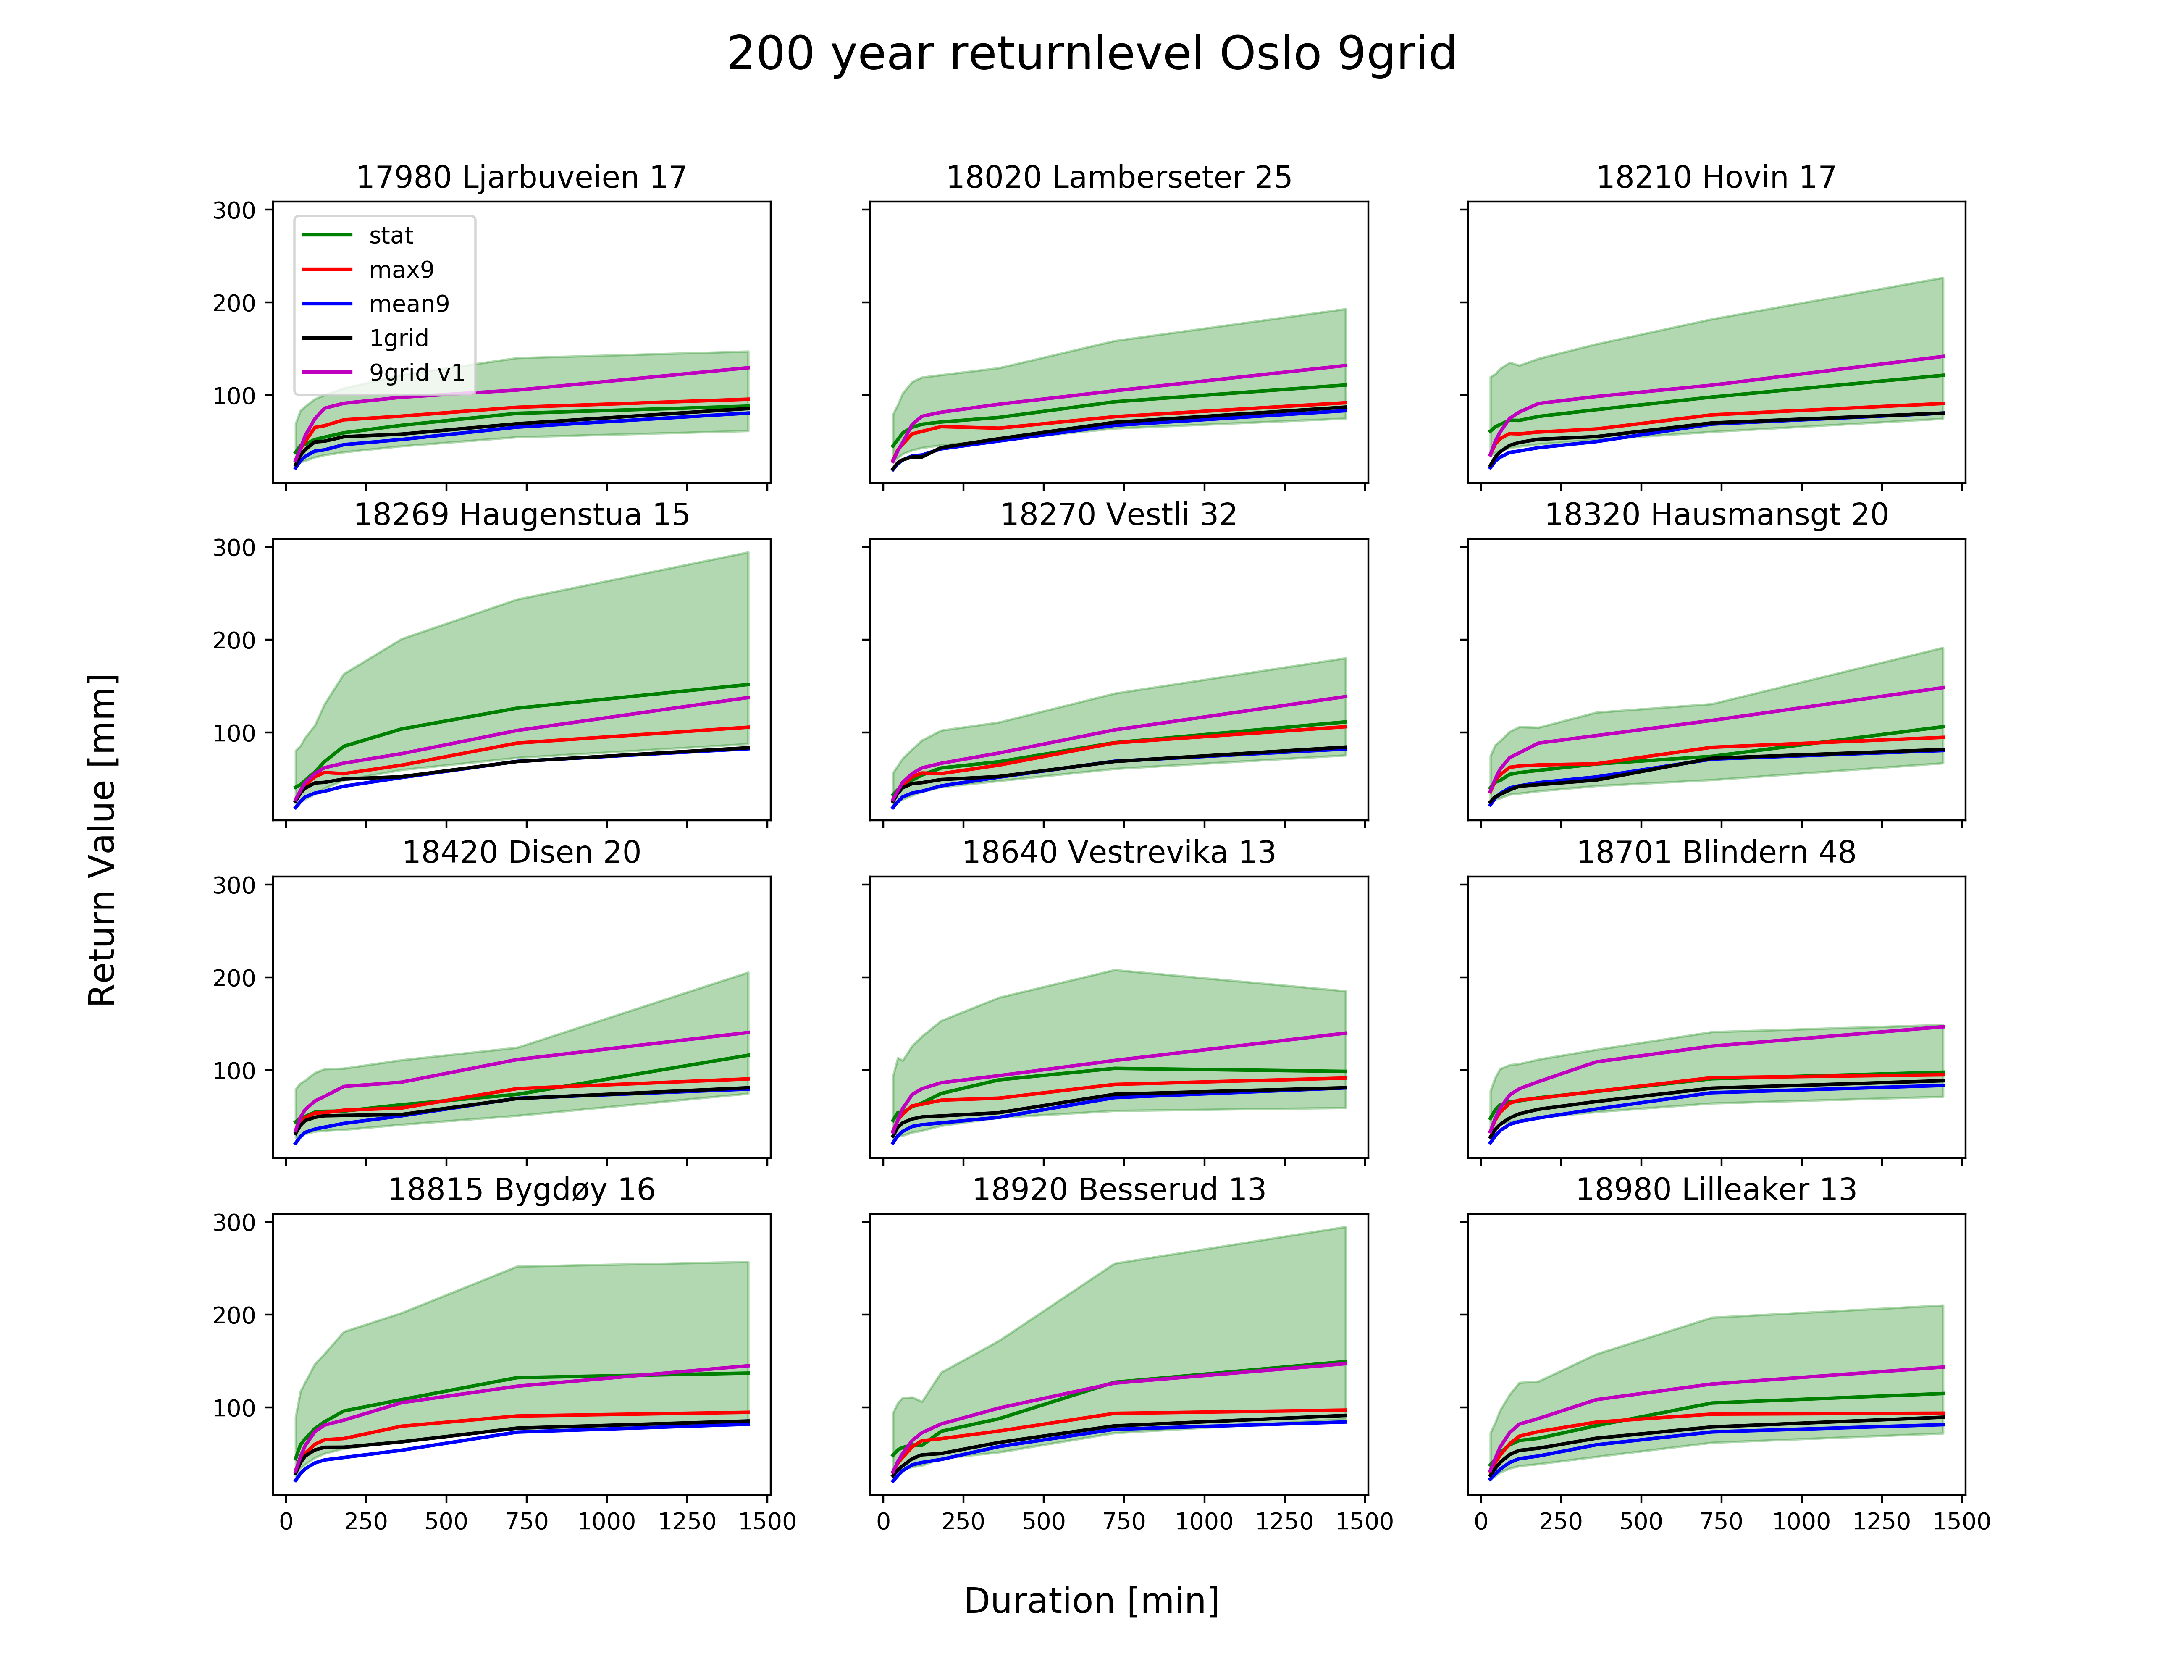
\includegraphics[scale=0.4]{figures/200_retper_ECE_1985_compare.png}
    \caption{Example figure. This is what I am talkin about
    \cite{lind_arome}}
    \label{fig:arome_domain}
\end{figure}

On average for all stations the $MAX$ method overestimate the IDF-values slightly for 2 year returnperiod, and slightly underestimate for all returnperiods larger than 5 years. In table \ref{dist_eval} the realtionship between the respective model and the station-based returnvalues are listed in station- and duration-averaged percentage. For station Haugenstua, Ljabruvegen, Hovin and Besserud it is close to identical to the $STAT$ method for all durations on the 2 year returnperiod. For the larger returnperiods it is the overall method closest to the $STAT$ method, esepecially for the stations with narrow confidence intervals. Providing higher estimates of the returnvalues than the $MEAN$ and the $1GRID$ method but smaller estimates compared to the $9GRID$ the $MAX$ method serves as a middle ground which according to table \ref{dist_eval} is more consistent with the station-based estimates on average for all the Oslo stations. Only for a 200 year returnperiod the station average for the $9GRID$ method is more consistent.        

\begin{table}[hbt!]
\centering
\begin{tabular}{ c c c c c}

Duration & 1grid & 9grid & mean9 & max9 \\
2 & 88.78 & 134.92 & 89.30 & 107.89\\
5 & 82.27 & 125.45 & 79.57 & 100.00\\
10 & 79.29 & 121.10 & 75.09 & 96.37\\
20 & 77.02 & 117.78 & 71.65 & 93.60\\
25 & 76.39 & 116.86 & 70.70 & 92.84\\
50 & 74.66 & 114.33 & 68.07 & 90.73\\
100 & 73.20 & 112.20 & 65.83 & 88.95\\
200 & 71.93 & 110.36 & 63.89 & 87.42
\end{tabular}
\caption{Station- and duration-average returnvalues for each returnperiod in percentage of the station-based station- and duration-average returnvalues. Each column is one method. Values >100 means averge overestimation copared to to the station-based values and values <100 mean underestimation.}
\label{dist_eval}
\end{table}


Even though we (I and Malte) agreed on not using the distance between the curves as any measure, it must be said that the "ax9" method now gives far better overall results compared to the stat.

\subsection{Intensity plots}

Precipitation intensity are in some cases more applicable than precipitation amount. In Figure \ref{fig:intensity_blindern_10} the 10 year return-level precipitation intensity is plotted for all durations and all AM methods at Blindern station. The intensity level difference is largest for small durations, decreasing to very small differences between the AM methods at 24 hours. At around 44mm/h the STAT method has the largest value at 15 minutes duration, while the MEAN method measures around 28  mm/h. Marked with the dotted lines in Figure \ref{fig:intensity_blindern_10} the 97.5 percentile value at 15 minutes is almost identical for STAT, MAX9 and 9GRID at approximately 55mm/h. 9GRID quickly turns into the method with largest intensity, also being the only method with a distinct intensity at 24 hours compared to the other methods. MAX has slightly higher intensity for all durations except 15 minutes compares to STAT, but are overall very similar. From 1 hour duration all methods except 9GRID and MEAN are within the confidence interval of STAT. On smaller durations 9GRID and MAX are the only to within the confidence levels of STAT.  

\begin{figure}[hbt!]
    \centering
    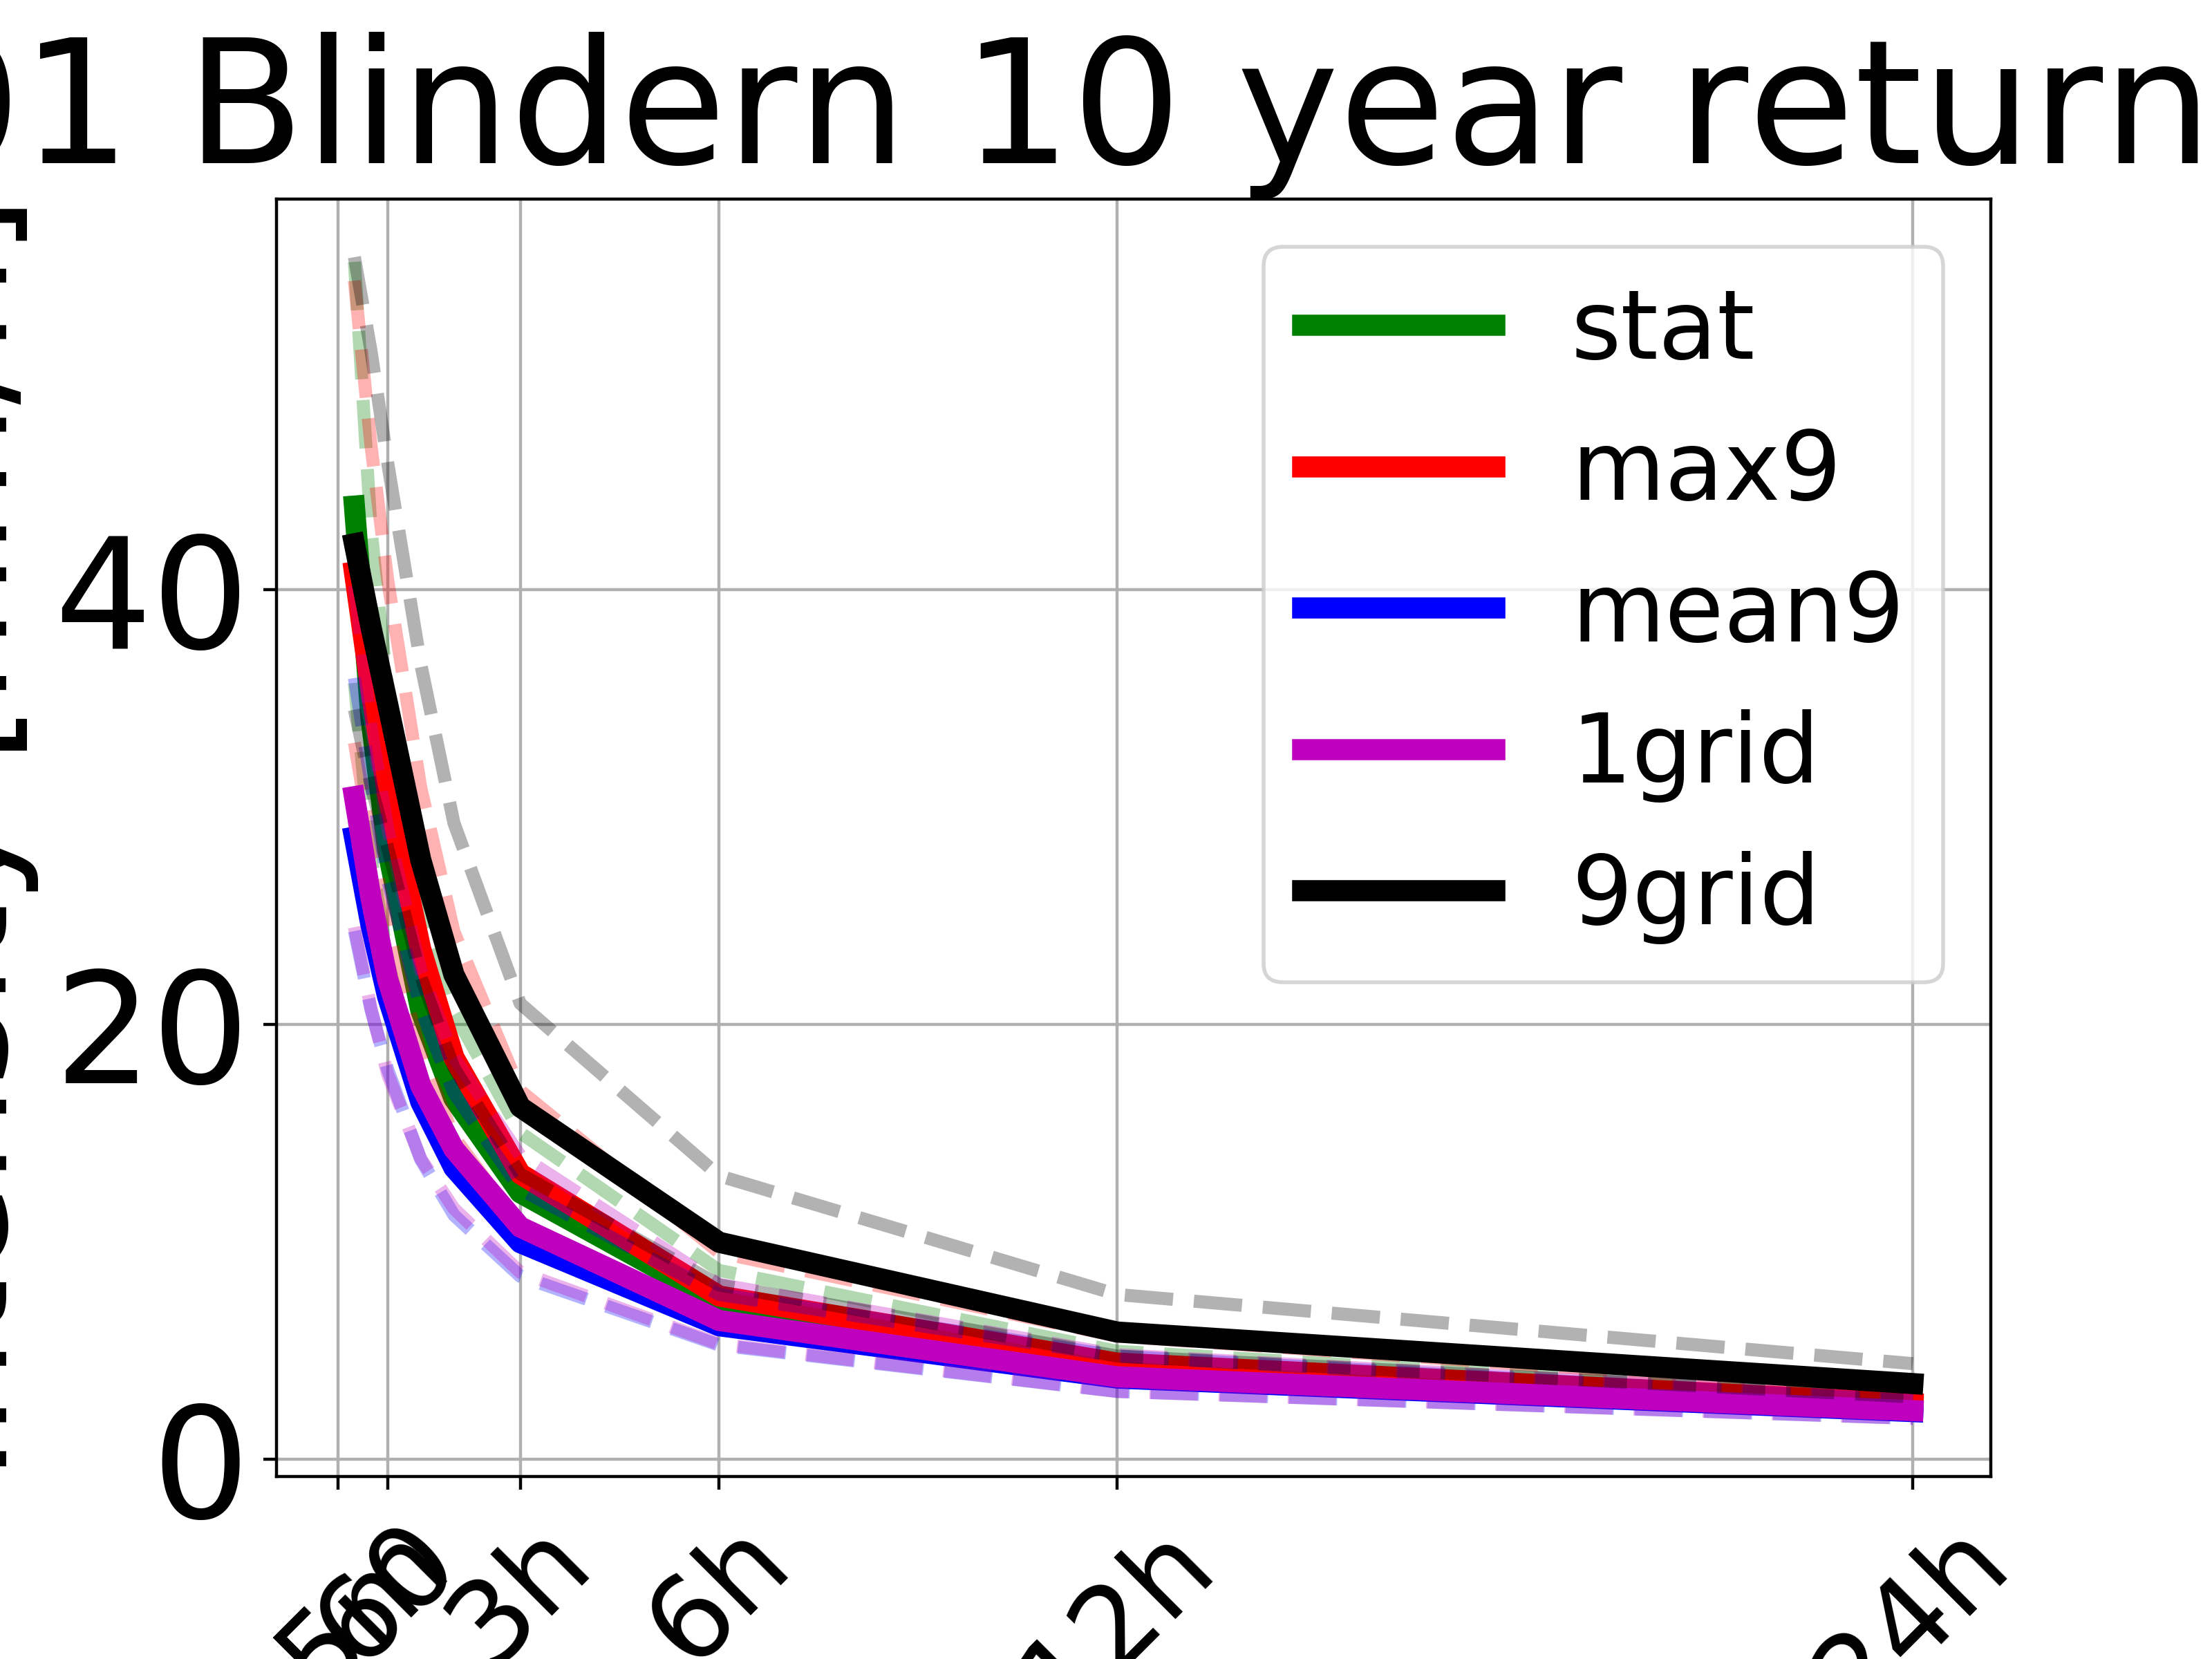
\includegraphics[scale=0.3]{figures/ECE_1985_real_idf_blindern.png}
    \caption{A caption.}
    \label{fig:intensity_blindern_10}
\end{figure}

Considering different return-levels a few features appears. Firstly, the STAT intensity and top/bottom percentile get increasingly larger compared to the other methods for short durations up to 1h with increasing return-period. This is probably due to the large confidence interval om the STAT compared to the modelled alternatives. For the 2 year return-period MEAN and 1GRID is the best fit to STAT intensity, while for increasing return-period up to 20 years the MAX method becomes increasingly closer to STAT for most durations. From 20 years onward the MAX intensity is very similar \textbf{close to identical for Blidnern)} to STAT for durations larger than 1 hour. As seen in Figure \ref{fig:intensity_blindern_200} \textbf{you also have this figure un-zoomed} 9GRID appears to have a gentler slope compared to the other methods as the return-period increases.  
\\
\\
\begin{figure}[hbt!]
    \centering
    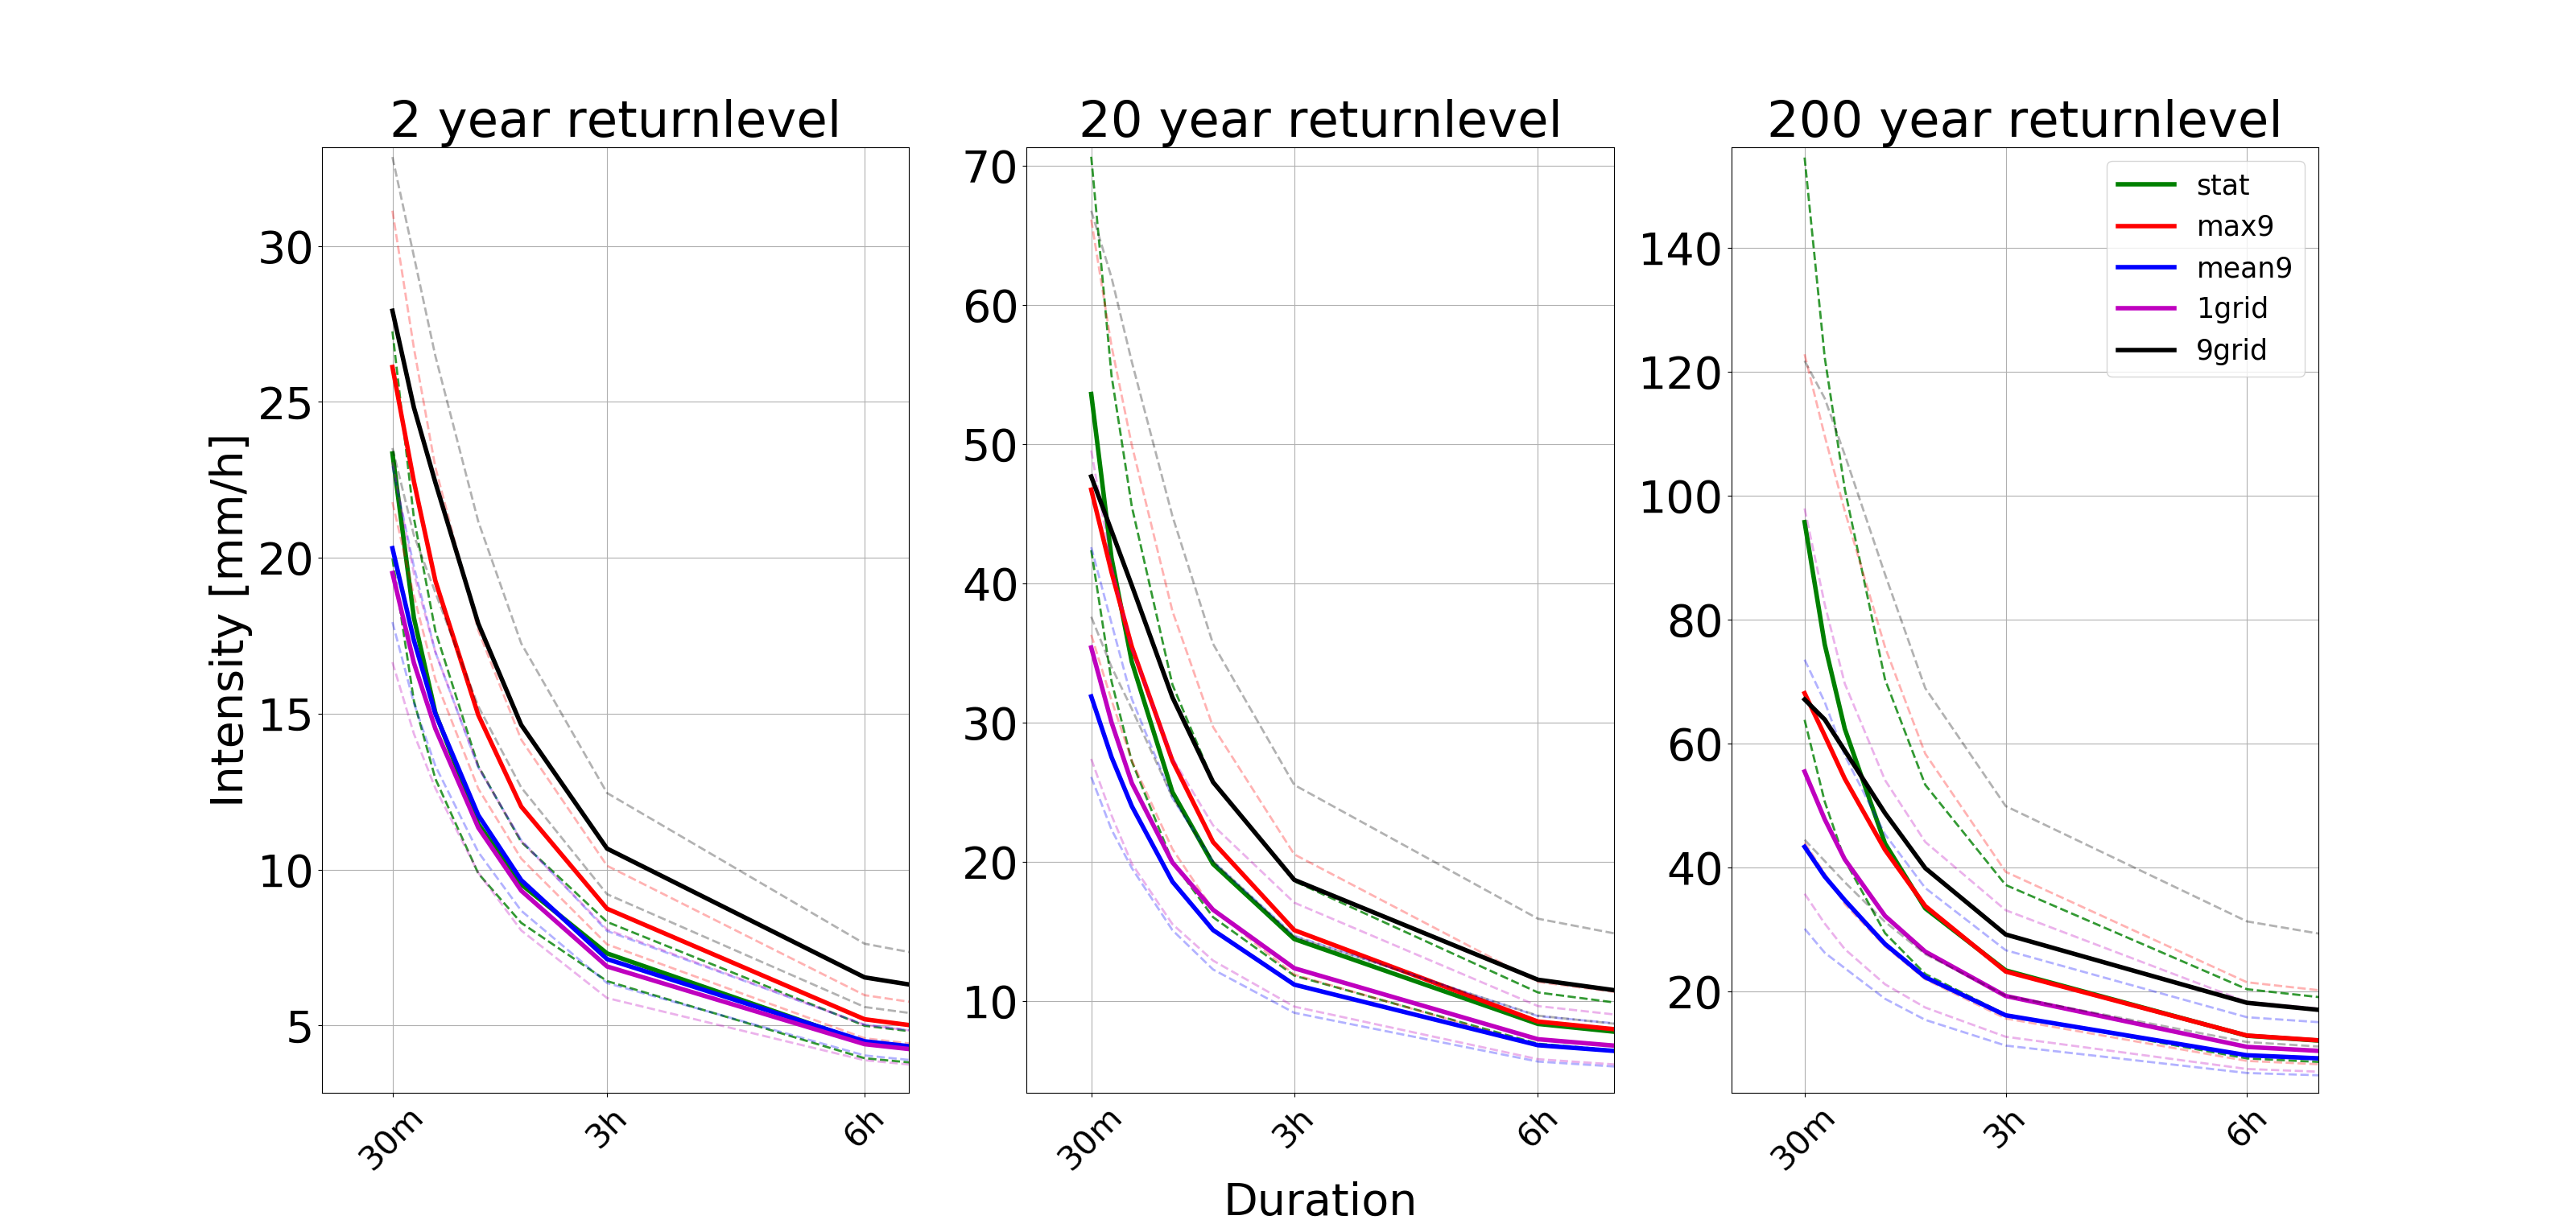
\includegraphics[scale=0.1]{figures/ECE_1985_2_20_200_zomed.png}
    \caption{A caption.}
    \label{fig:intensity_blindern_200}
\end{figure}
\\
\\
\textbf{commenting on figure from max-mean-evaluation of 2, 20 and 200 year return levels Blindern.} Evaluating the return-levels in Figure \ref{fig:idf_blindern_2_200} instead of intensity reveals some other features. From Figure \ref{fig:idf_blindern_2_200} one can observe that the MEAN and 1GRID are the only methods inside the STAT confidence interval for the 2 year return-period. For all other return-periods MAX is also well within the STAT confidence interval. At 50 year return-period 9GRID is included in the STAT confidence interval from 30 min to 6 hours duration. At 100 years RP it is included until around 18 hours duration, while at 200 RP 9GRID is within the STAT confidence for all durations. However, for all RP 9GRID is a round 50 \% larger than STAT at 24 hours duration. Similarly to Figure \ref{fig:intensity_blindern_200} (check if its the correct figure, the one wigh 2-200), Figure \ref{fig:idf_blindern_2_200} reveals that for small RP STAT is very equal to MEAN and 1GRID, while it becomes closer to MAX as the RP increases.

\begin{figure}[hbt!]
    \centering
    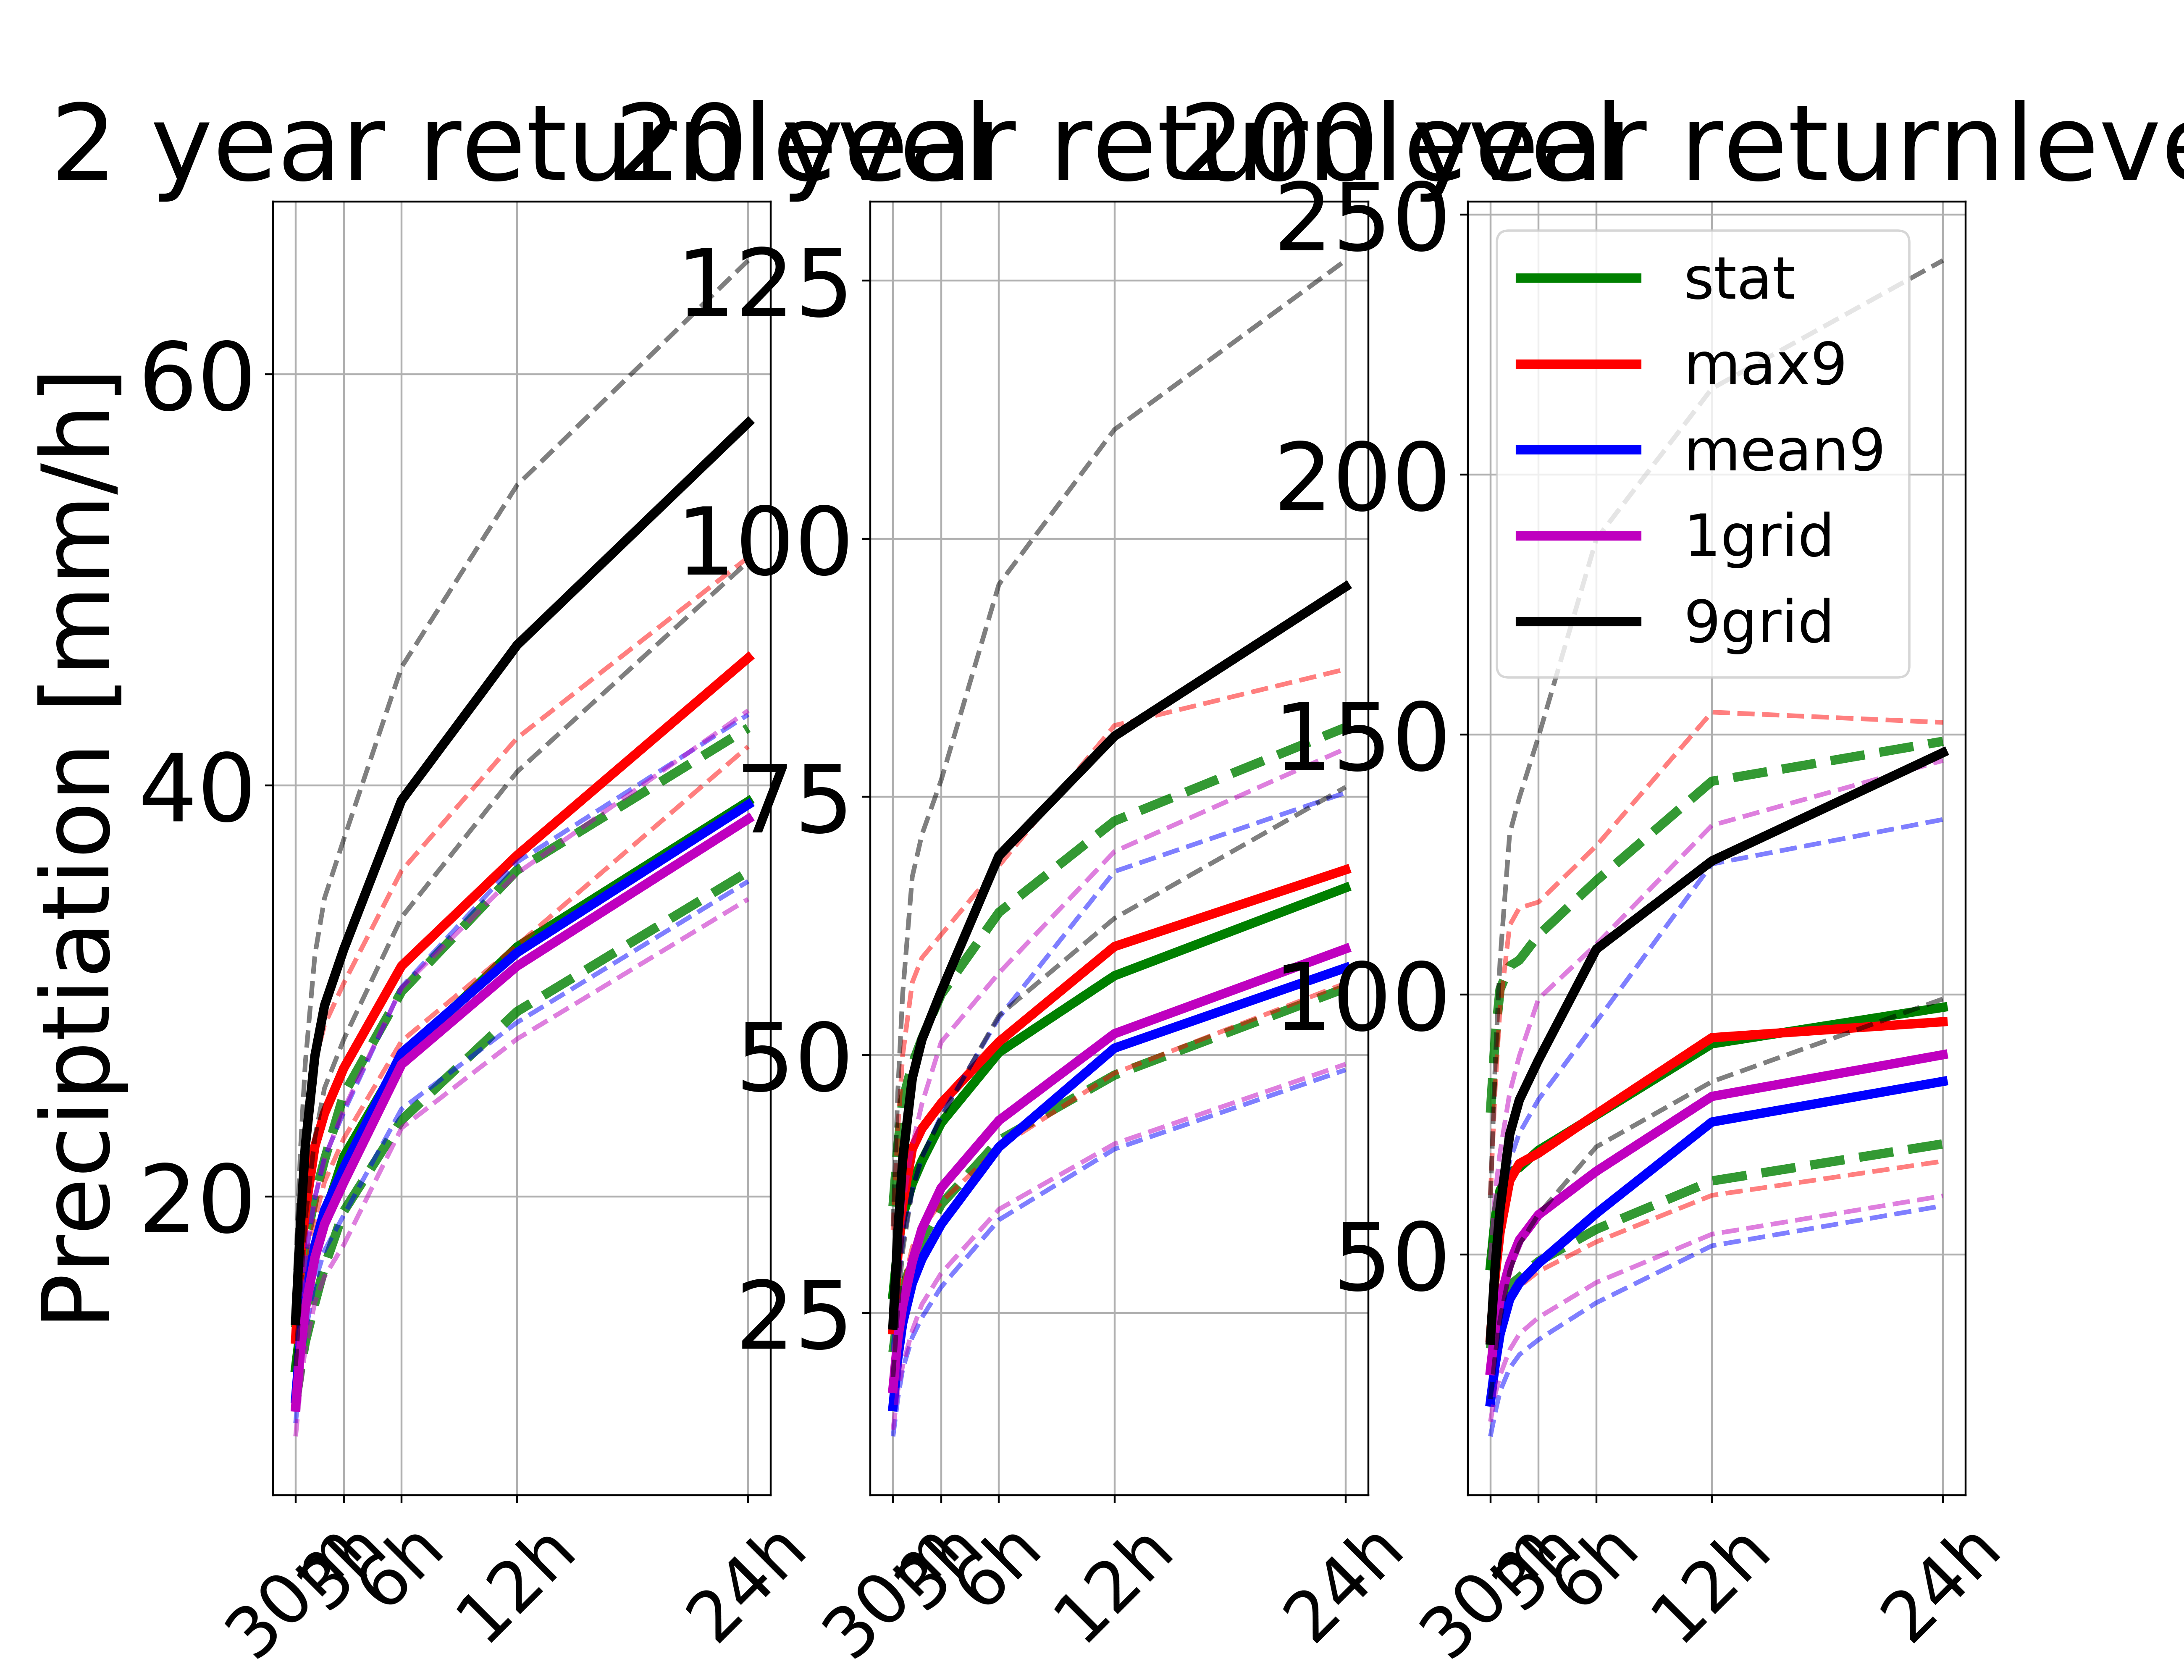
\includegraphics[scale=0.4]{figures/ECE_1985_idf_blindern_2_20_200.png}
    \caption{A caption.}
    \label{fig:idf_blindern_2_200}
\end{figure}

Another feature of the precipitation magnitude curves from Figure \ref{fig:idf_blindern_2_200} is the enormous confidence intervals, especially at large RP. Already at at 20 year RP the 95 \% confidence interval for 6 hour duration is 42 to 66 mm, and at 24 hours duration its around 60 to 125 mm. Bearing in mind this is the Blindern station with the longest, 48 year, data-series, these confidence intervals are large. For short durations the MEAN confidence interval is close to that of STAT, while on the longer durations MAX is closest on the 2.5 percentile and the MAX and 1GRID is closest on the 97.5 percentile. For all return-periods the 9GRID top-percentile is sky-high and way above any other values. \textbf{Mayby include an example from another station as well, which does not look "as good" as Blindern?}
\textbf{comment somewhere on the shape of the curves. Why are they steep in the beginning and then smoothening?}

\textbf{connet the following with the table above with percentage differnce from STAT} To investigate how the AM methods performs for the entire Oslo area the station- and duration IDF average precipitation amounts for all 12 stations and all listed durations from 30 minutes to 24 hours are calculated for each return-period. The result is displayed in Figure \ref{fig:table_dur_stat}. In panel A the 9GRID duration- and station average is the only method producing values larger than STAT. Both STAT and 9GRID are increasing at approximately the same rate with increasing return-period, around 0.24 mm/year on average. The MEAN and 1GRID method both have smaller values compared to STAT, increasing at around 0.14 mm/year. The MAX method are very similar to STAT for 2,5 and 10 years, then underestimating it slightly towards the larger RP. With increasing precipitation magnitude of around 0.20 mm/year In panel B of Figure \ref{fig:table_dur_stat} the individual curves from panel A are plotted as percentage of the station- and duration average STAT precipitation magnitude value. MAX method has the smallest average deviation from STAT for all RP except 200 years, where the 9GRID has the smallest deviation. \textbf{not sure if both panels is really necessary. can skip one of them an shorten the text a bit here.}      

\begin{figure}
    \begin{center}
        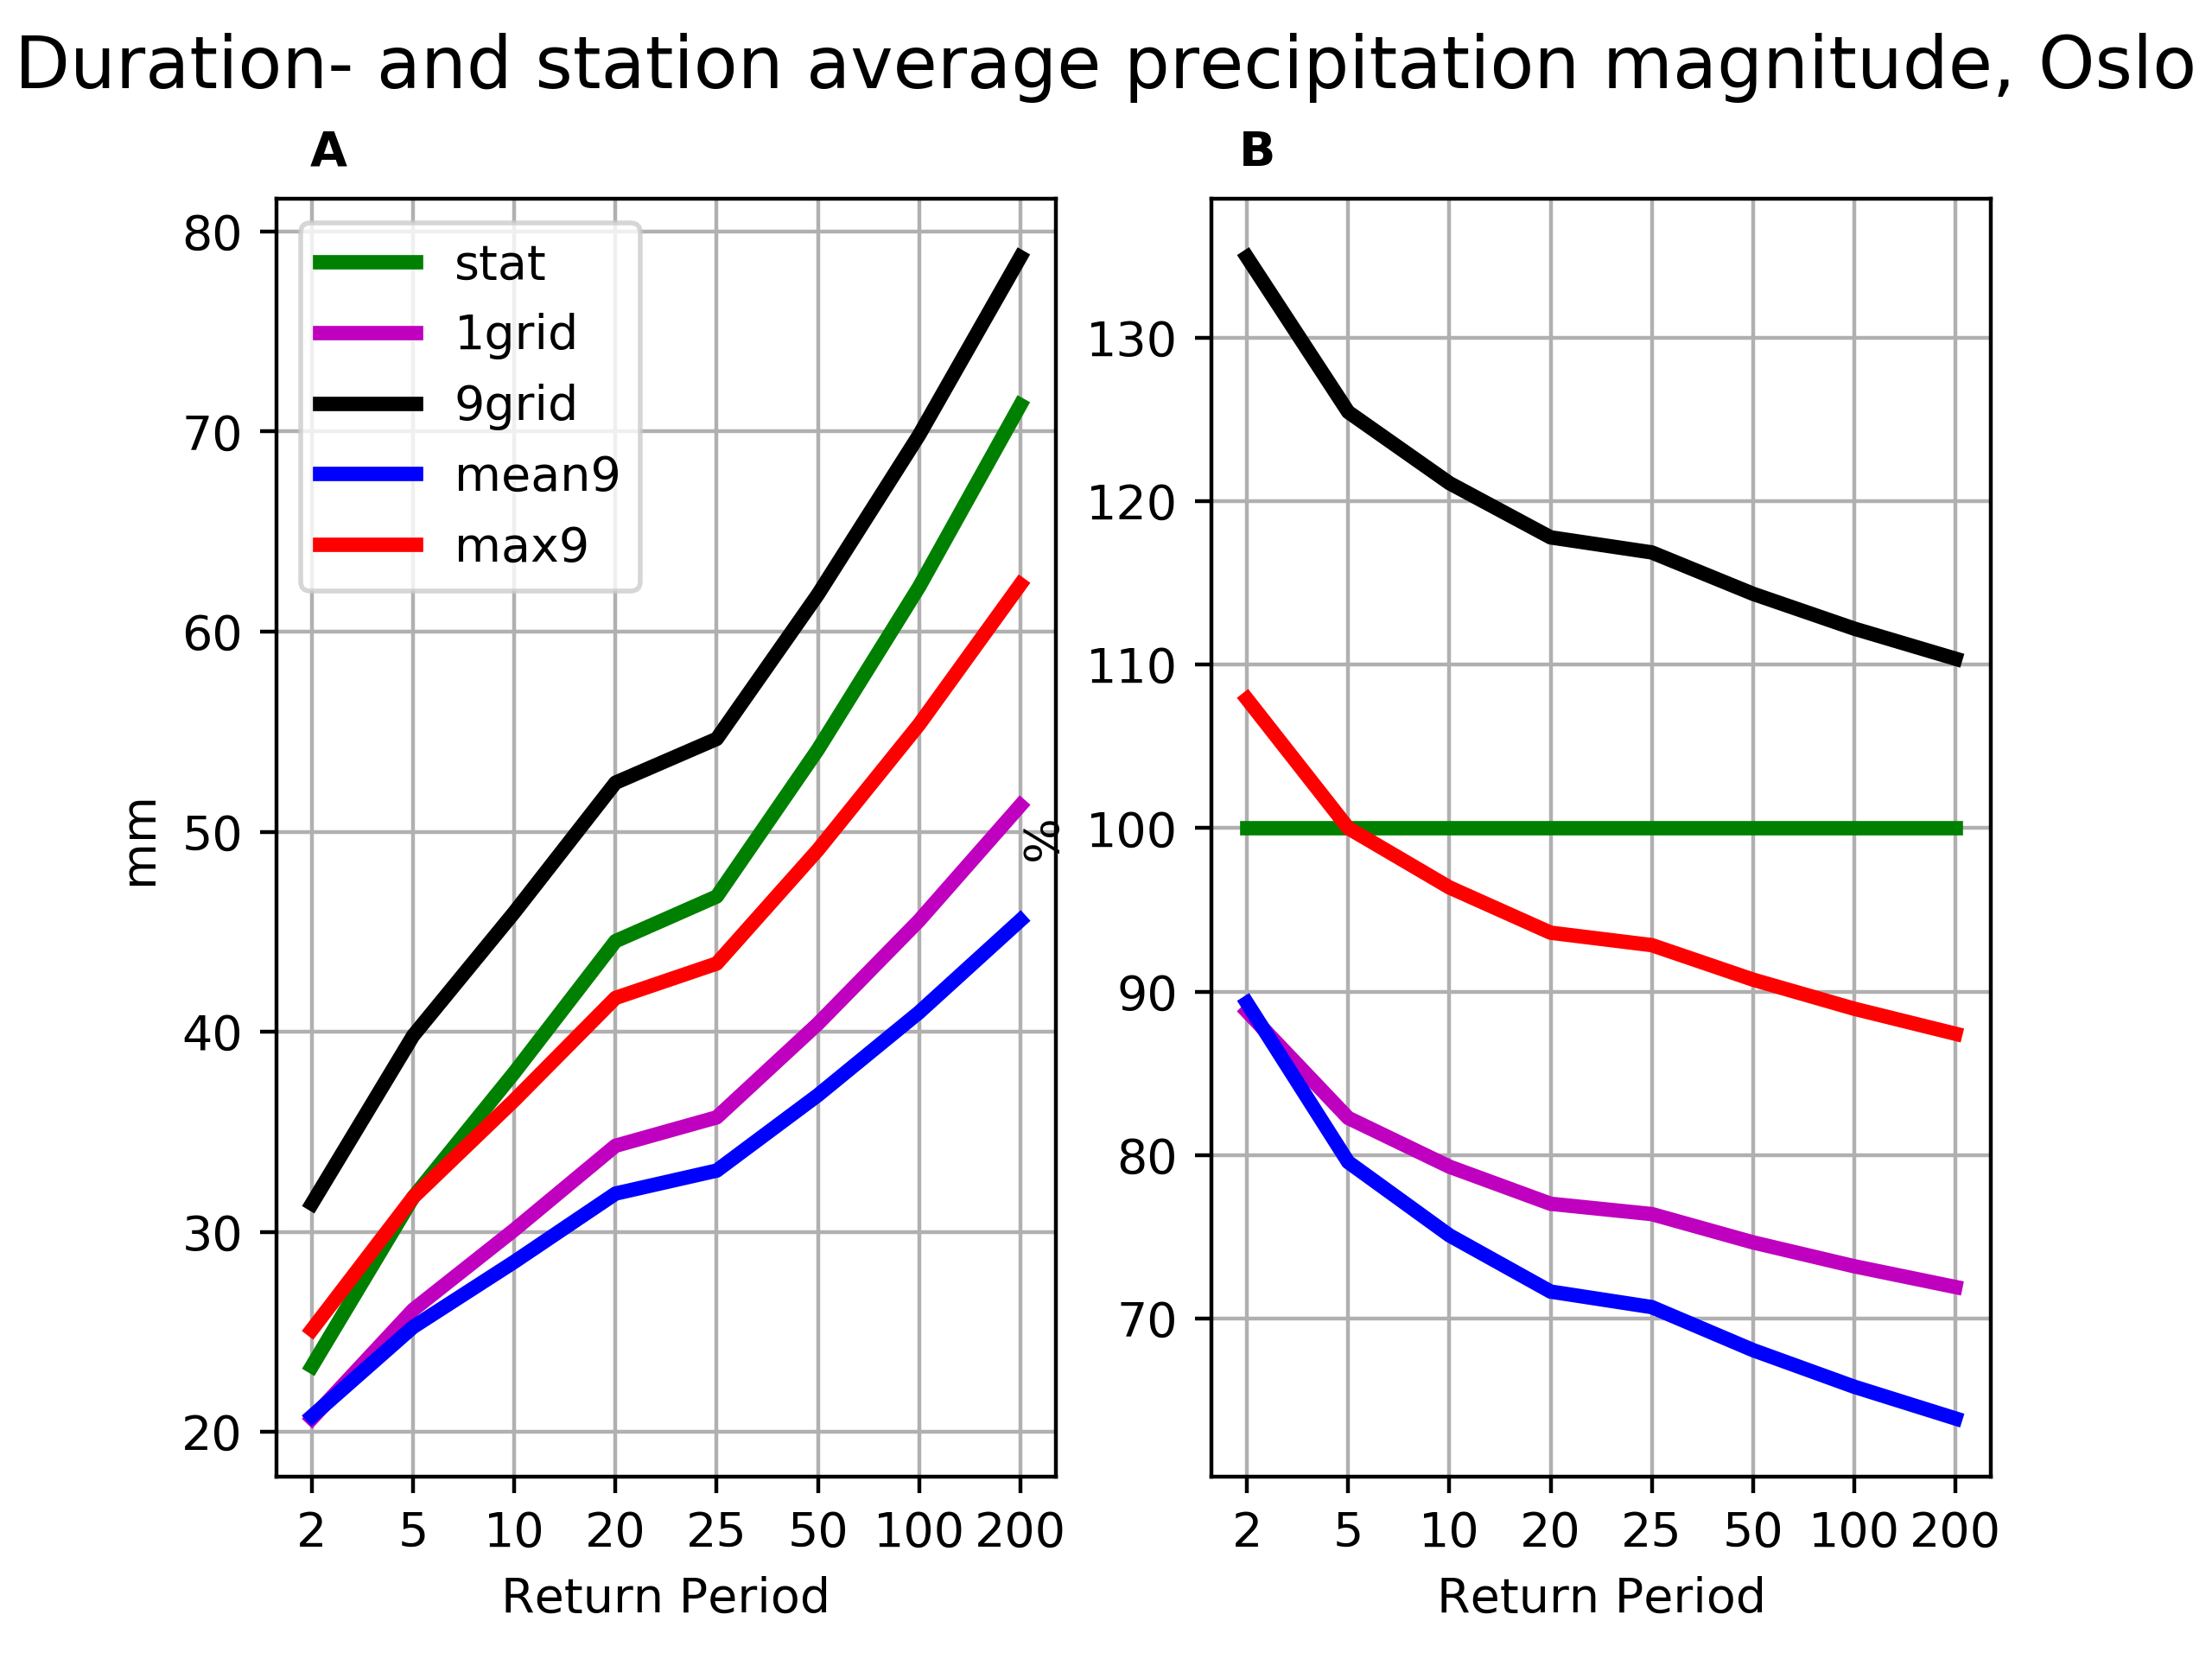
\includegraphics[scale=0.4]{figures/table_avg_dur_stat.png}
    \end{center}
    \caption{A PGF histogra.}
    \label{fig:table_dur_stat}
\end{figure}

Despite their close proximity, the precipitation values for a given return-period varies substantially amongst the stations. Figure \ref{fig:1985_all_stat} displays 10 year return-values for all stations and AM methods. The shaded green area indicates the 95 \% cofidence interval for STAT. As indicated by the number after each station name, the STAT data-series length for the specific station varies. For the two stations with longest data-series, Blindern and Vestli, 9GRID is outside STAT top percentile, thus overestimating the return-level. The confidence interval Blindern and Vestli are also the smallest of the 12 stations. For stations like Lilleaker, hovin, Lamberseter and Disen 9GRID is right around the STAT top percentile, sometimes within and sometimes outside. For the Haugenstua, Bygdøy and Besserud station 9GRID is by far closest, and at times almost perfectly aligned with the STAT mean value. Common for these three is the relatively short STAT data-series length, with 15, 16 and 13 years respectively. For the other 9 stations MAX appears to provide the overall best fit. However, as the RP increases MAX is loosing its position as overall best "fit" to 9GRID for a few stations and durations.           

\begin{figure}
    \begin{center}
        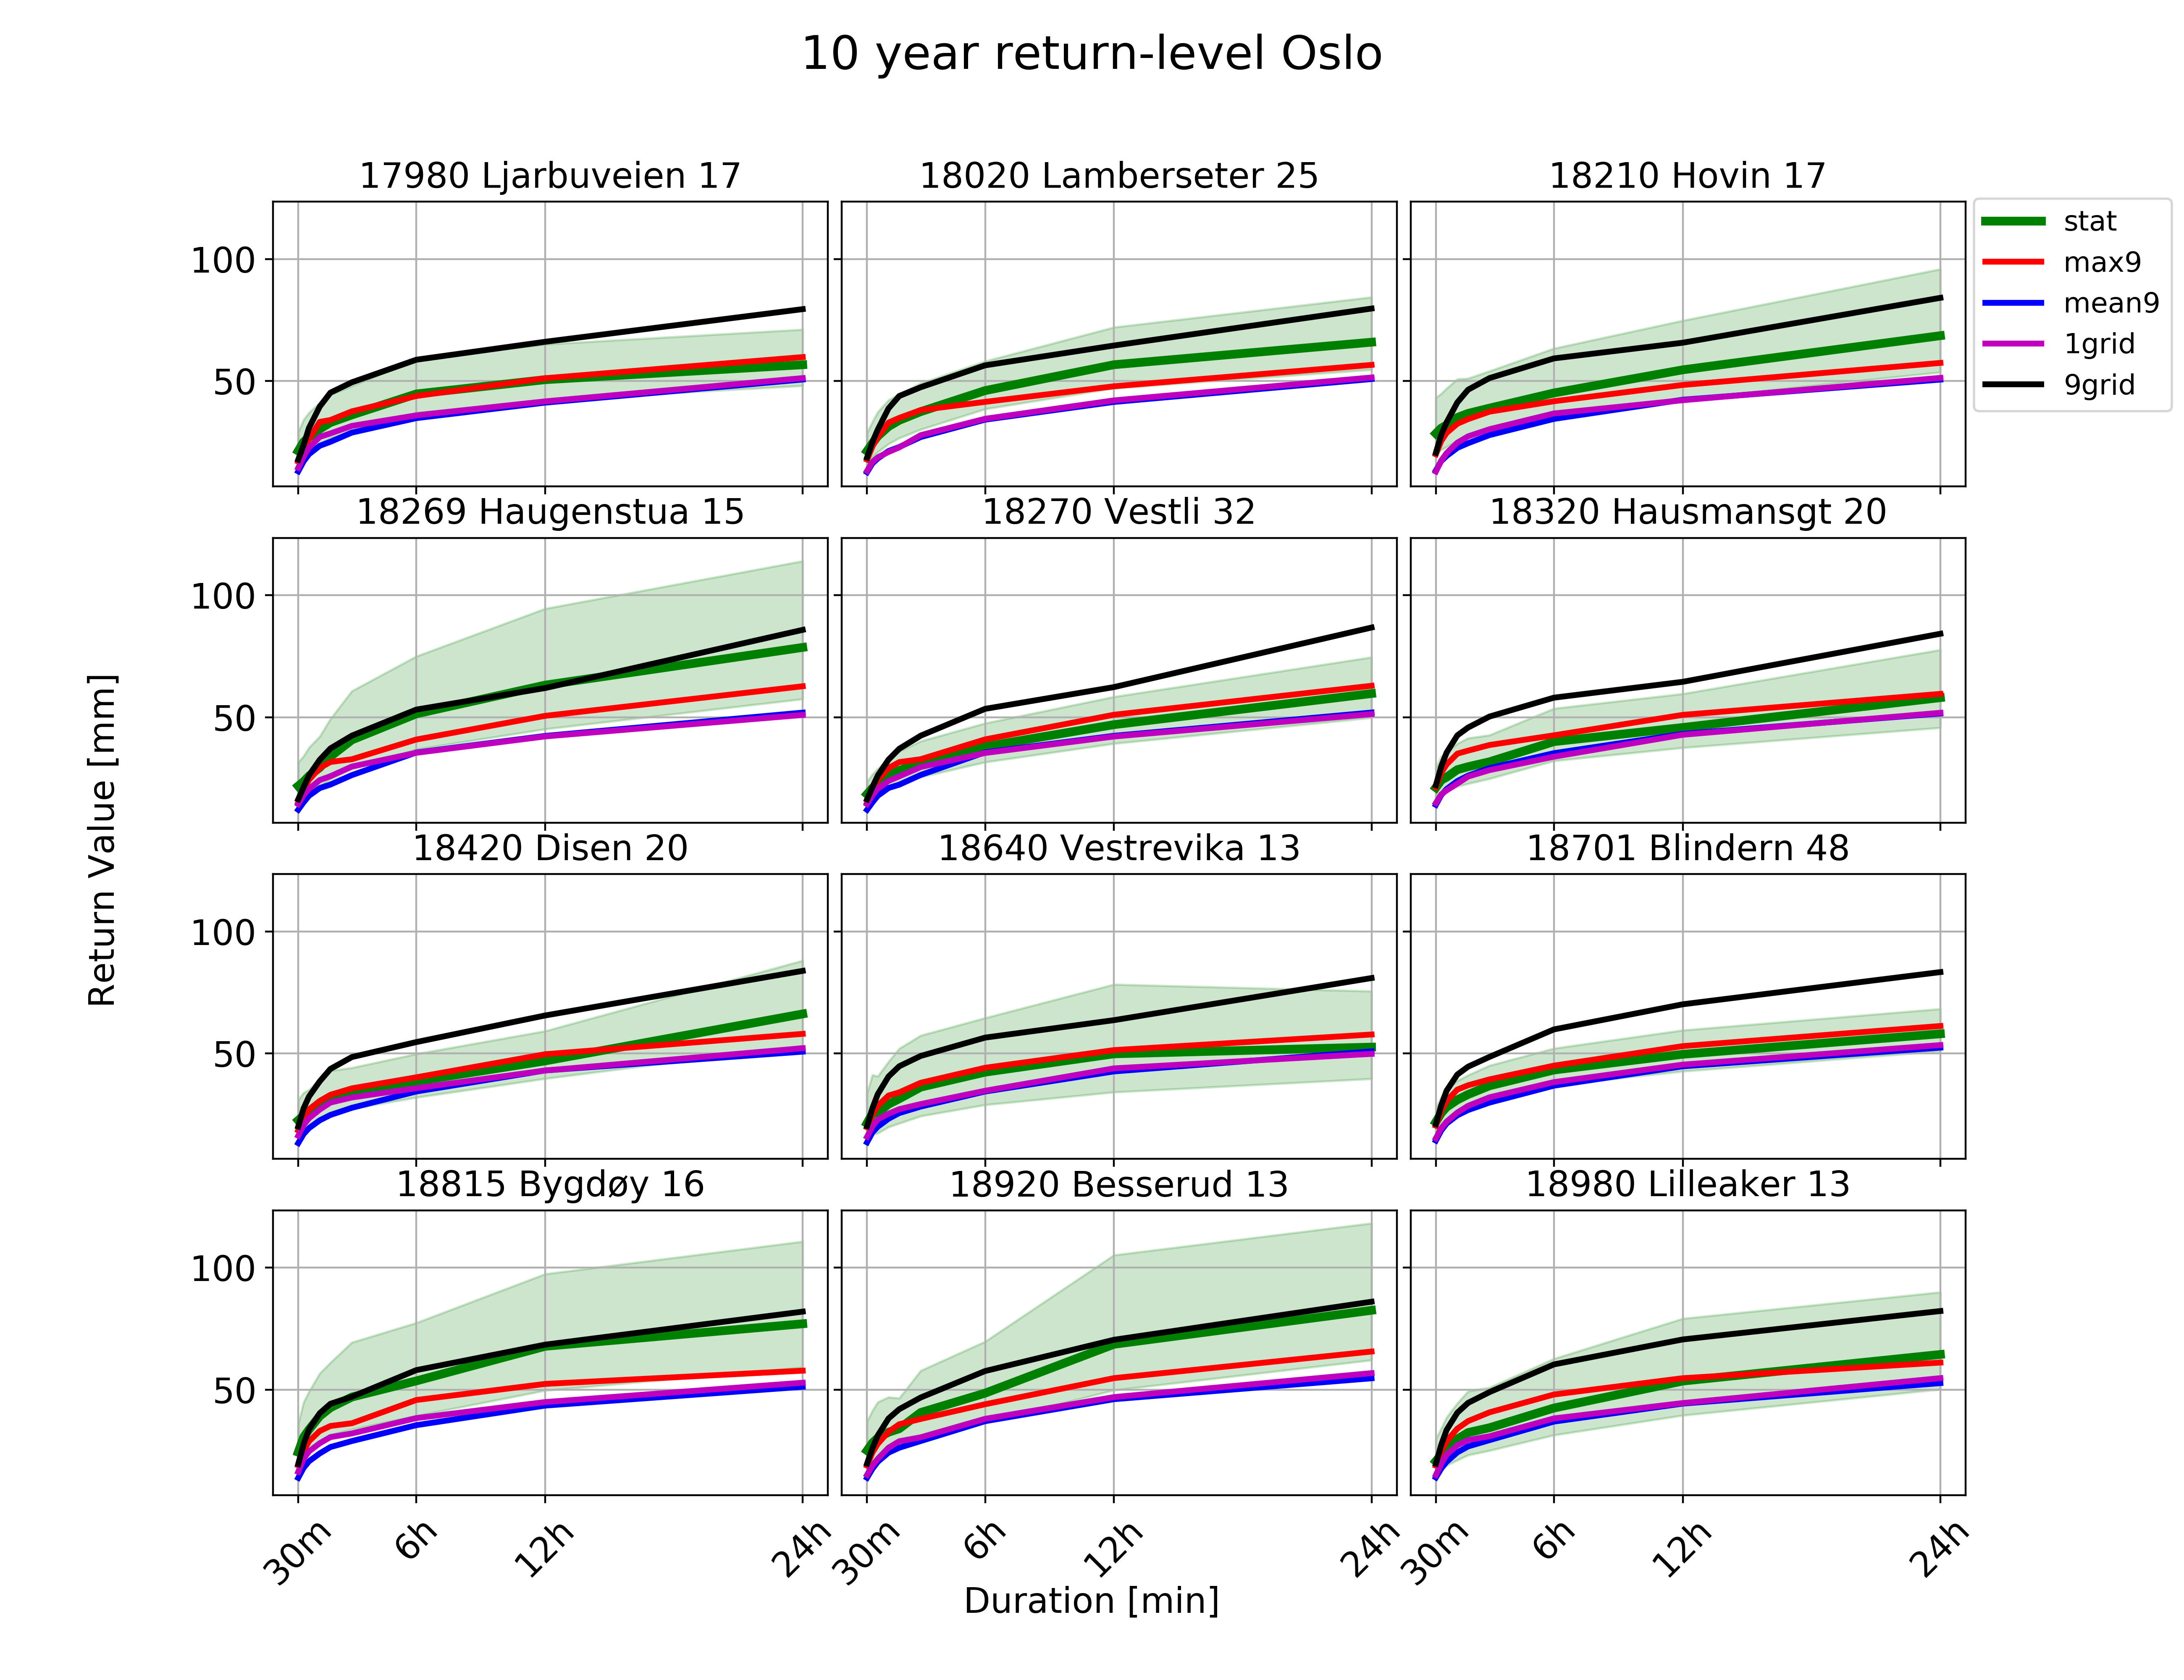
\includegraphics[width=20cm,height=8cm,keepaspectratio]{figures/10_ECE_1985_all_stat.png}
    \end{center}
    \caption{A PGF histogra.}
    \label{fig:1985_all_stat}
\end{figure}

The MEAN and 1GRID methods provide very similar return-levels for all stations and all RP. For 2 year RP they have the best fit to STAT at Blindern Vestrevika, Vestli and Hausmannsgate for all durations, but also to Lilleaker and Disen for durations smaller than 12 hours. 

\subsection{Annual Maxima}

Investigating how the annual maxima time-series of the stations and the model behave might provide information on the nature of the IDF values and their uncertainties. Figure \ref{fig:Am_stations} shows AM for all stations for 15 minutes and 24 hours duration for station 18701 Blindern. The black line are the mean AM precipitation value. Even though Figure \ref{fig:AM_stations} only show two of the durations, analysis show large variations in AM between stations across all durations for most stations. The spread for each yearly value seems to be quite large. A few years like 2003 and 2004 have available station AM values close to each other for all durations. This also apply to other years, but in most cases the number of data-points for those years are only 2-3. From 1968 to 1996 there are mostly three stations available each year. In this period some years have one or two stations available. Thus, four to five stations governs the AM pattern for all durations more than half of the total time-series length from 1968 to 2018. From around year 2000 the number of available stations each year increases. This also increases the spread in this years. Some stations have largest or highest AM value a specific year for some or all durations, but this is more not than often the case.      

\begin{figure}[hbt!]
    \centering
    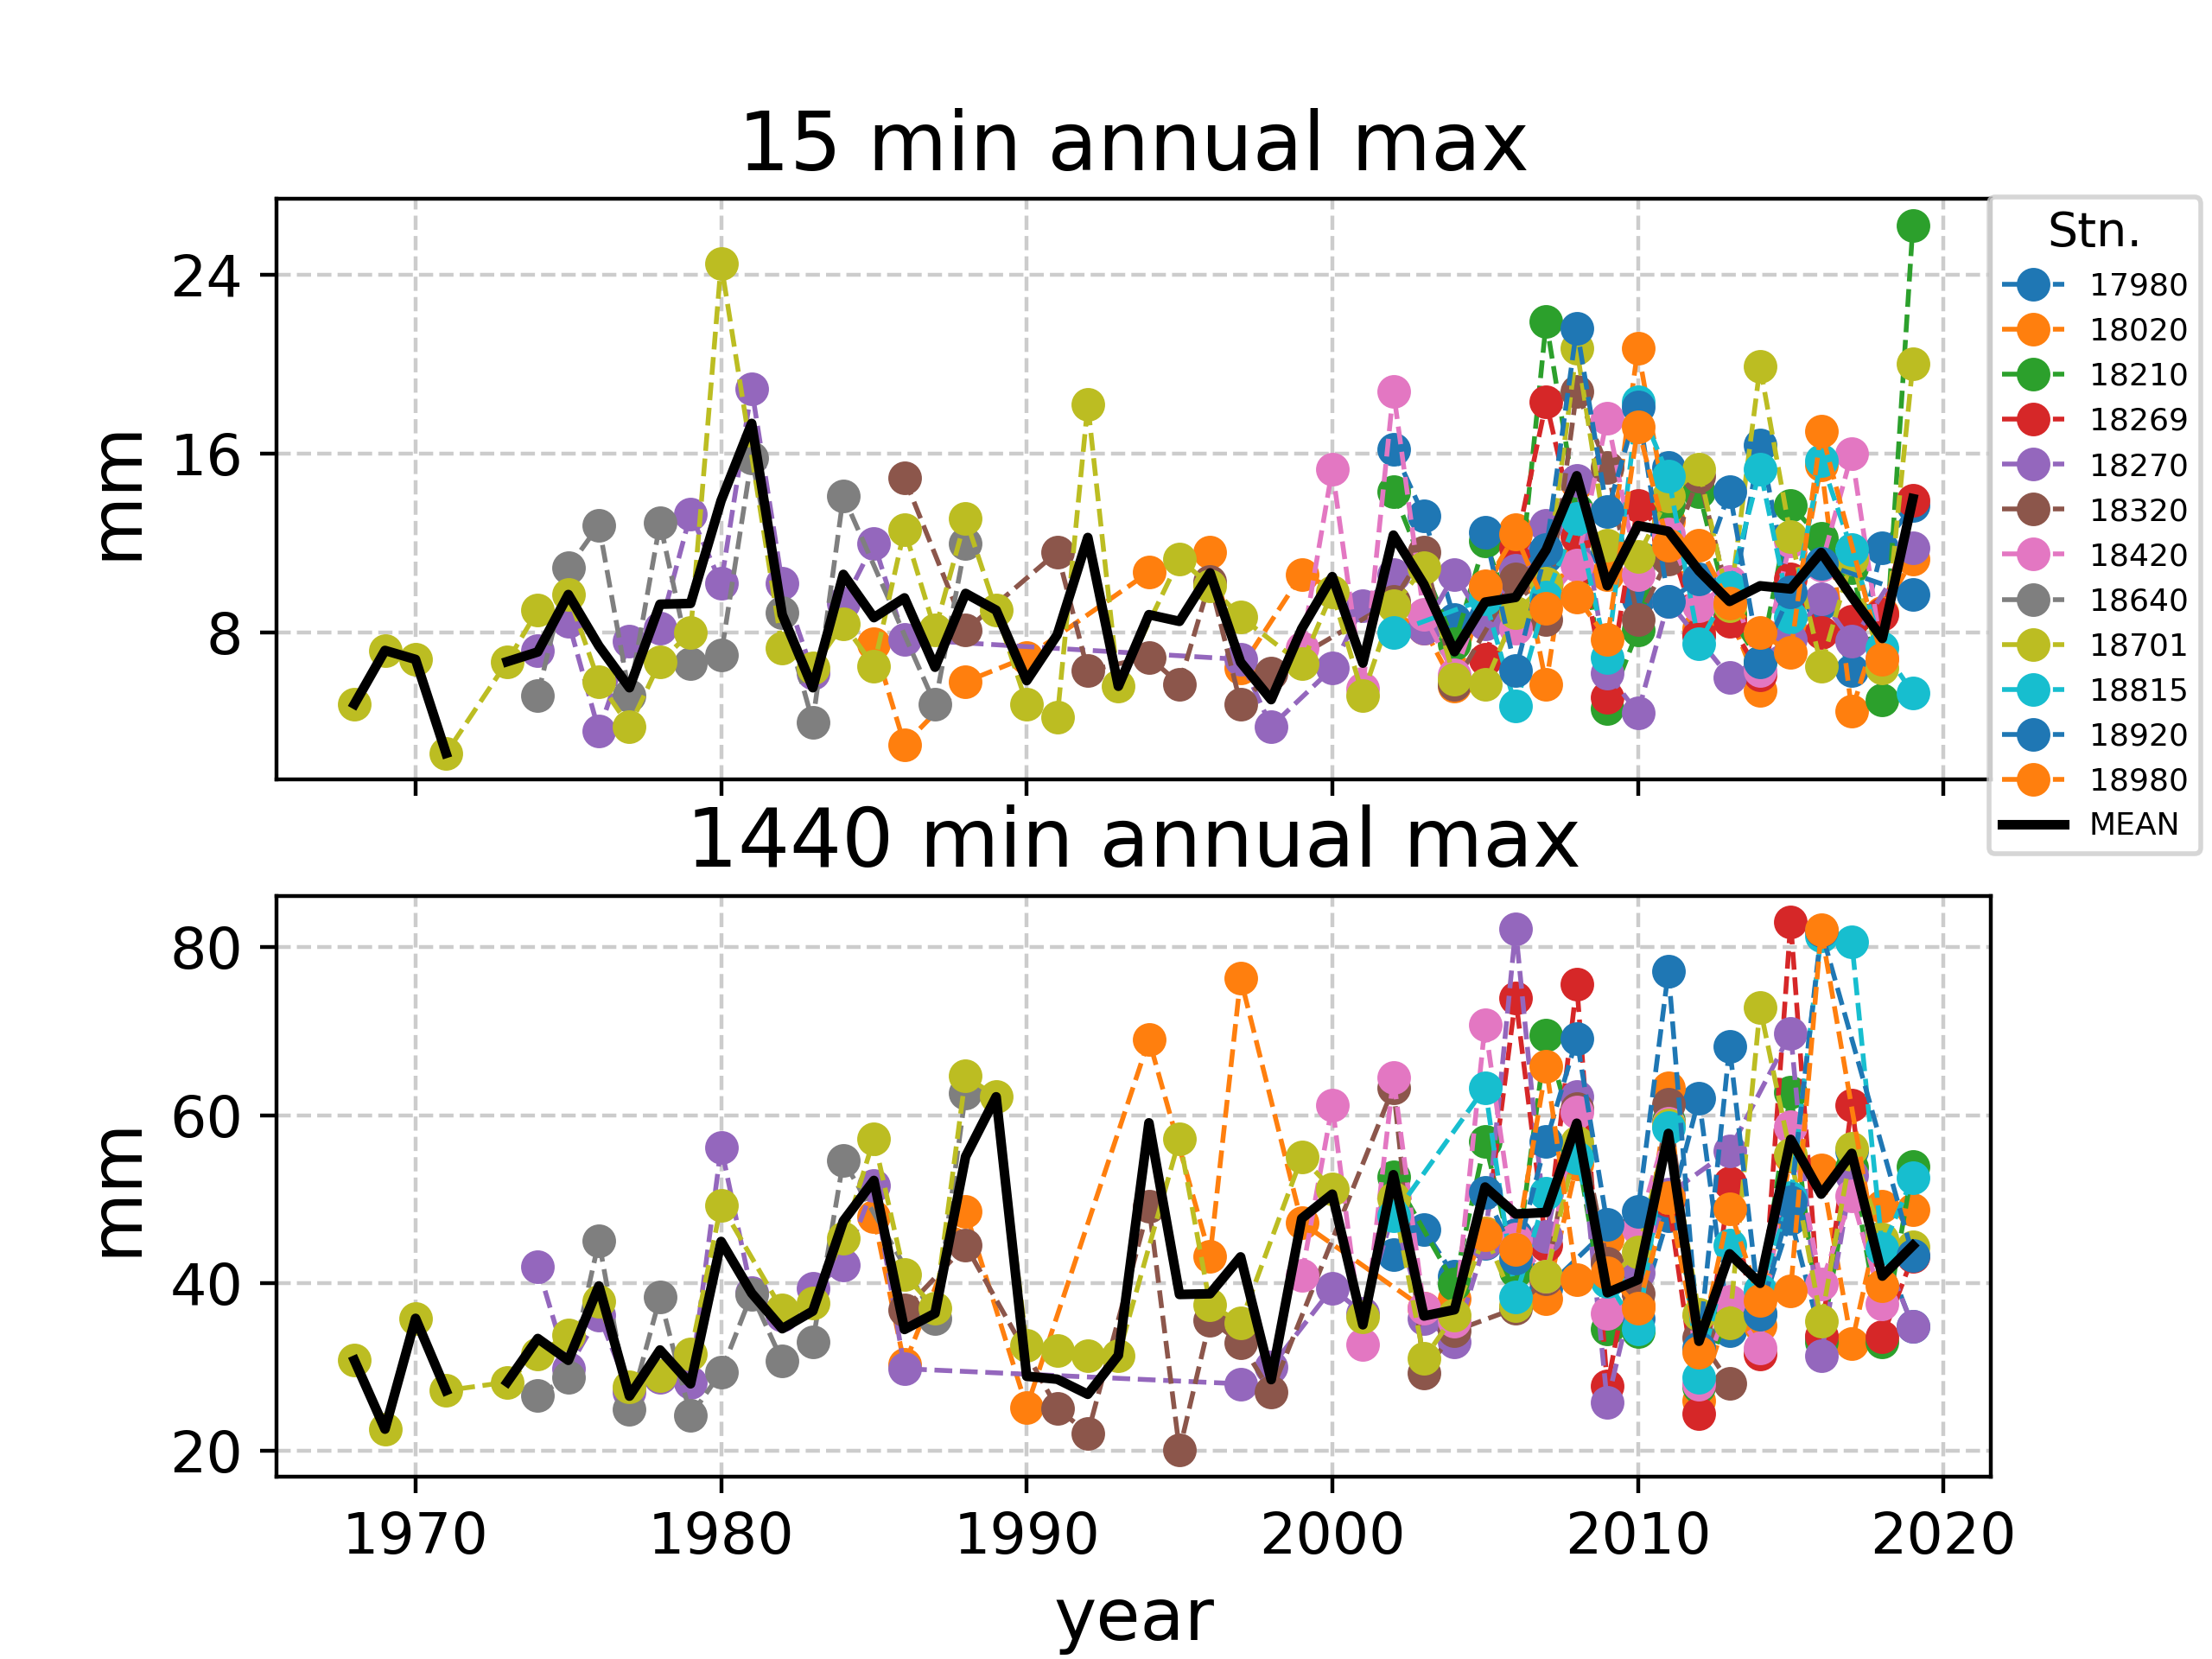
\includegraphics[scale=0.8]{figures/AM_stations.png}
    \caption{A caption.}
    \label{fig:AM_stations}
\end{figure}
\\
\\
Now we investigate how the modelled AM precipitation compares to the station AM. In Figure \ref{fig:AM_stat_mod} the station mean AM from Figure \ref{fig:AM_stations} is plotted with station average AM from the different AM methods for durations 15, 60, 360 and 1440 minutes from 1985 to 2005. The shaded gray area is one standard deviation (STD) of the station mean AM for the respective duration. The most noticeable feature is that the four methods used with the modelled precipitation overlap quite well with the station-curve. An exception that with longer duration the 9GRID method appears to fall increasingly far outside the 1 STD of the station-curve. For all durations 1GRID and 9MEAN AM are close to identical throughout the 20 years, while MAX falls between 9GRID and MEAN/1GRID. In periods like 1988-1992 and 1995-2000 most durations up to 360 minutes the modelled AM and the station-based AM agree very well, while the durations 360 minutes and larger have a good agreement between the model and the measurements in the period 1989-1995. For almost all years and duration one or more of the modelled methods are within the standard deviation of the measurements. However a few exceptions exists, like the year 2001 where all modeled AM methods are outside the measurement STD for durations up to 360 minutes. Another noticeable feature is that the 9GRID method appears to increasingly overestimate the AM values with increasing duration. This might suggest hat the method is not very well suited for IDF calculations, especially for the larger durations.   

\begin{figure}[hbt!]
    \centering
    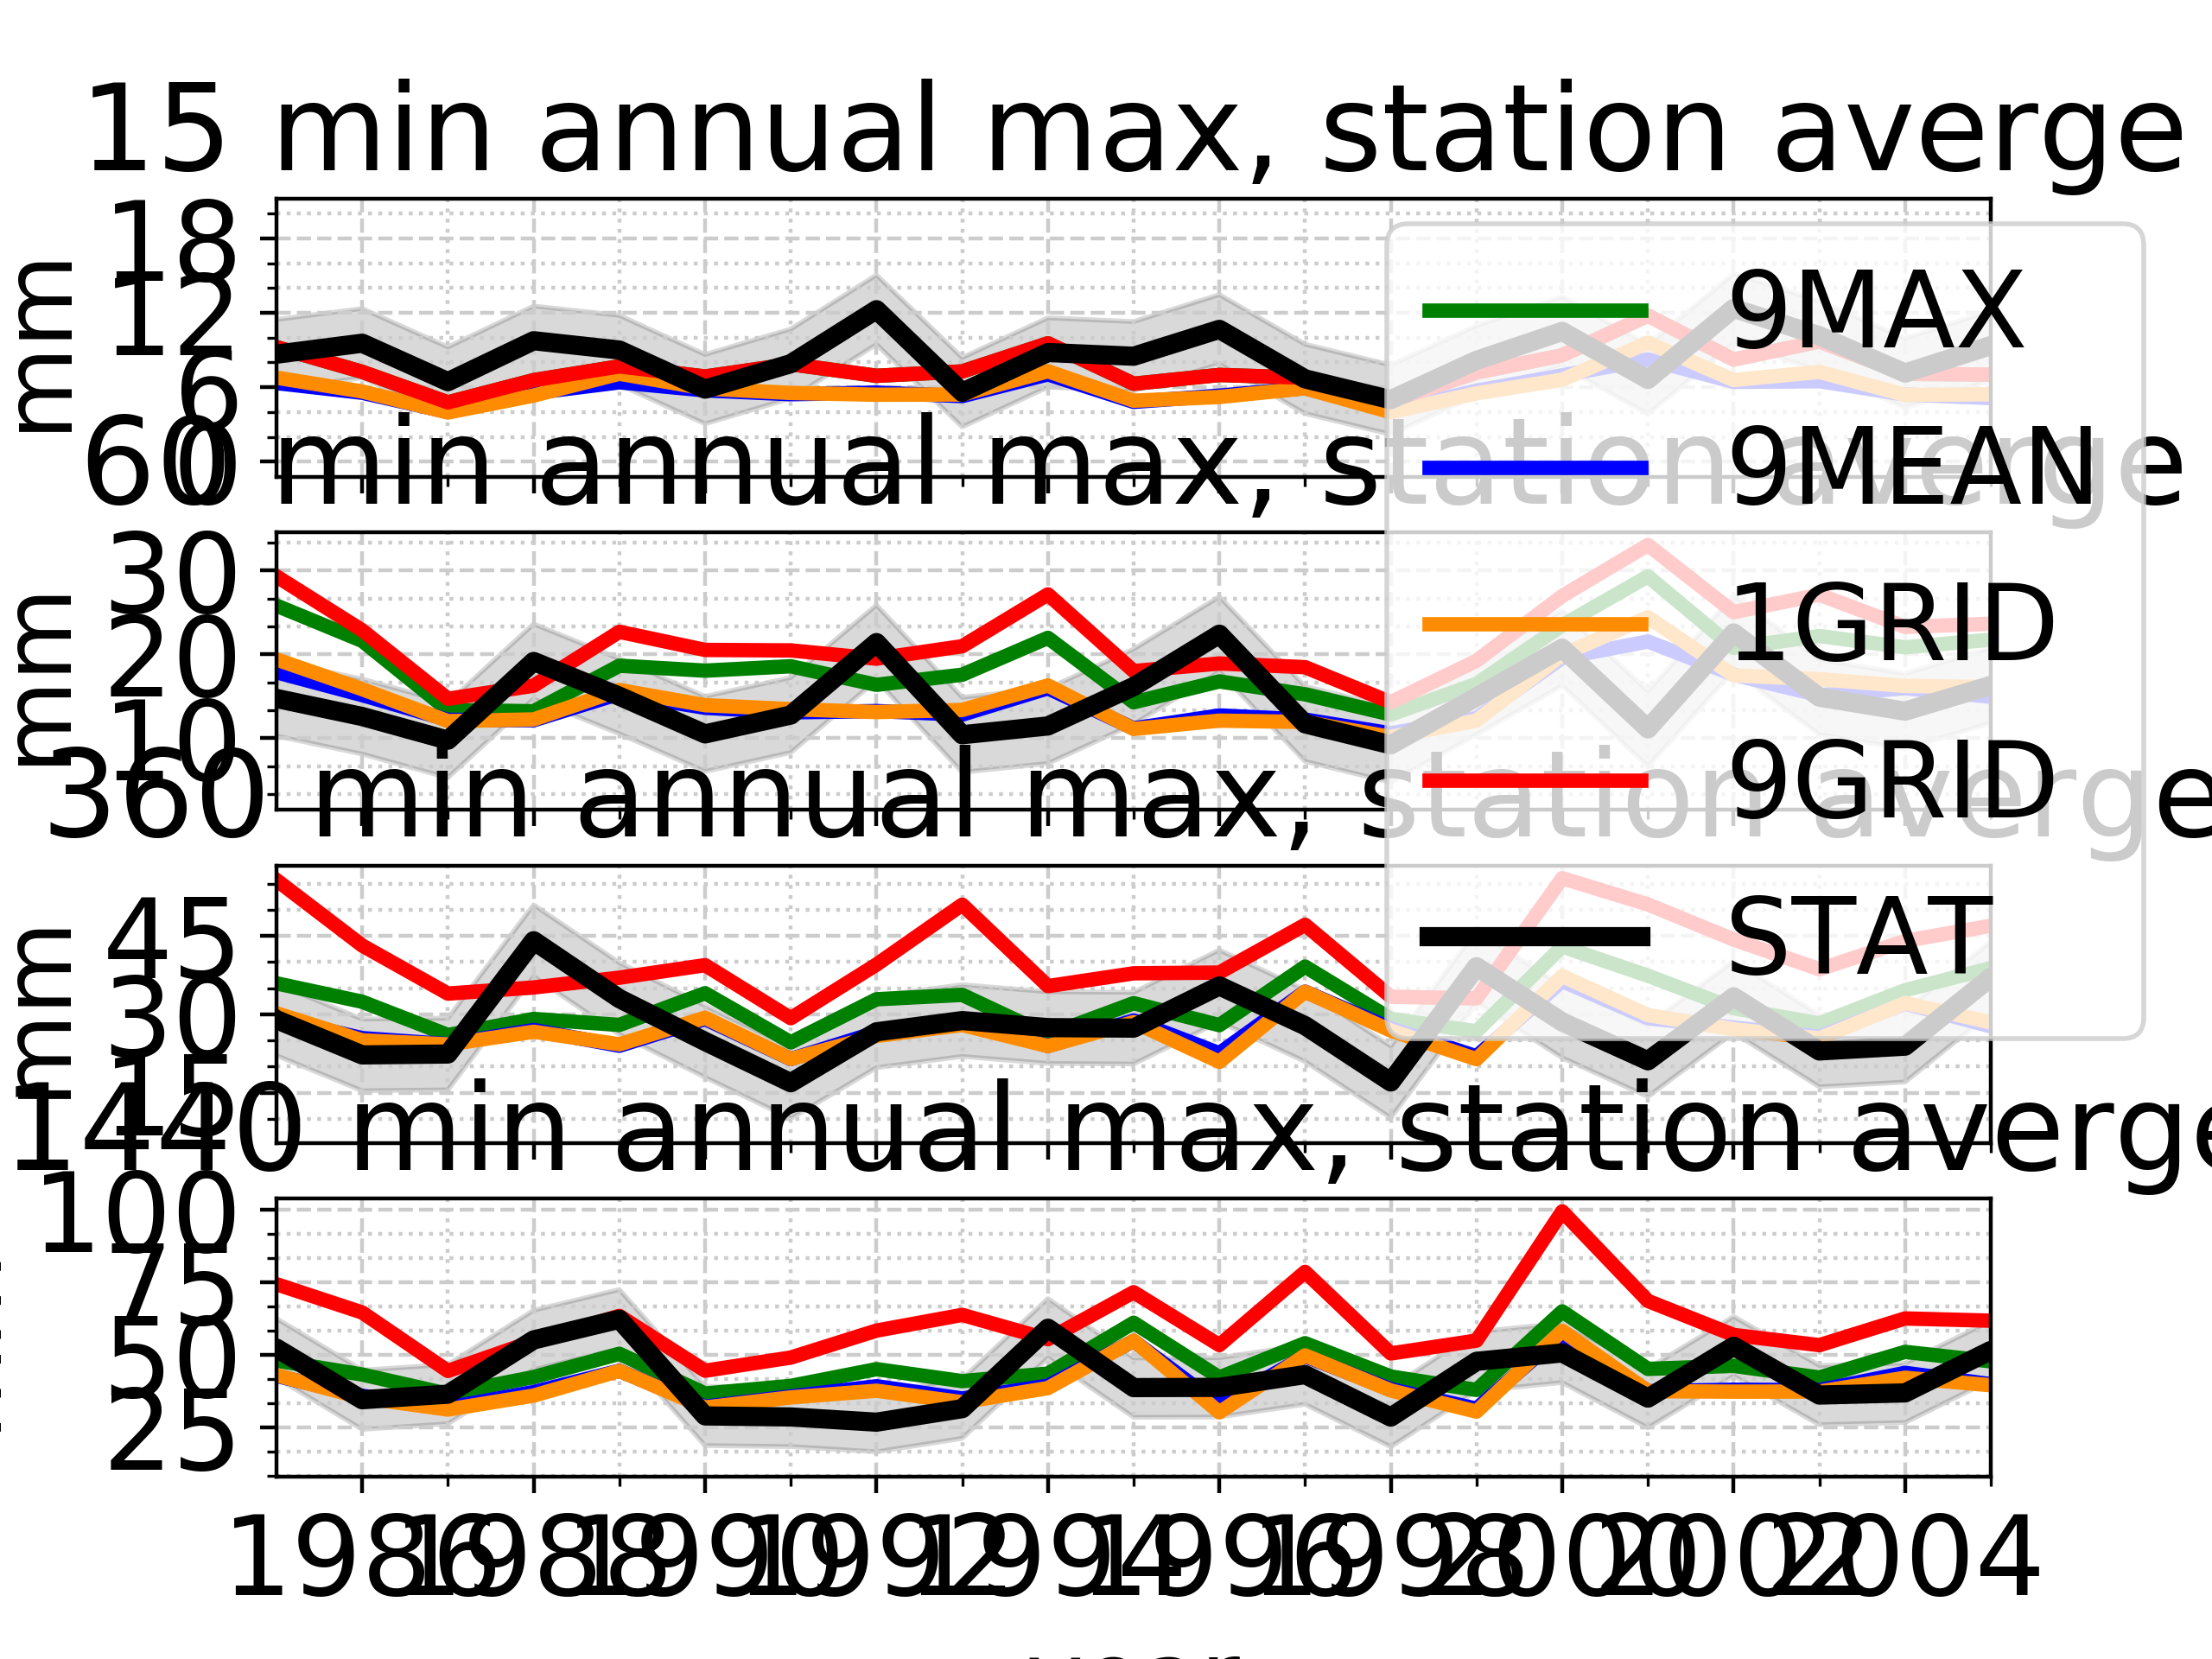
\includegraphics[scale=0.8]{figures/AM_stat_mod.png}
    \caption{A caption.}
    \label{fig:AM_stat_mod}
\end{figure}
\\
\\
Annual maxima differs substantially between the methods for the individual stations and durations. The variations in AM could partially account for the spread in the resulting IDF-curves. In Figure \ref{fig:AM_dur} a heatmap of the duration average variance of annual maximum precipitation for each station and each method is plotted. The number within the parenthesis on the y-axis refers to the time-series length of the station-data. For the other methods the time-series length is 20 years for all stations. The most noticeable feature is the large range of variance on the station-based data compared to the other method. Large variance indicates large spread, and hence the year to year difference in annual maxima is larger for the station data compared to the modelled data. Station 17980 Ljabruvegen has the smallest STD at XXX while station 18815 Bygdøy has the largest STD at for the station-based annual maxima. It is also noticeable how the STD for stations like 18701 Blindern and 18020 Lambergseter with long time series is on the high end of the scale amongst these stations. At the same time short time-series stations like 18980 Lilleaker, 18920 Besserud and 18640 Vestre Vika also have high relative STD.  

\begin{figure}[hbt!]
    \centering
    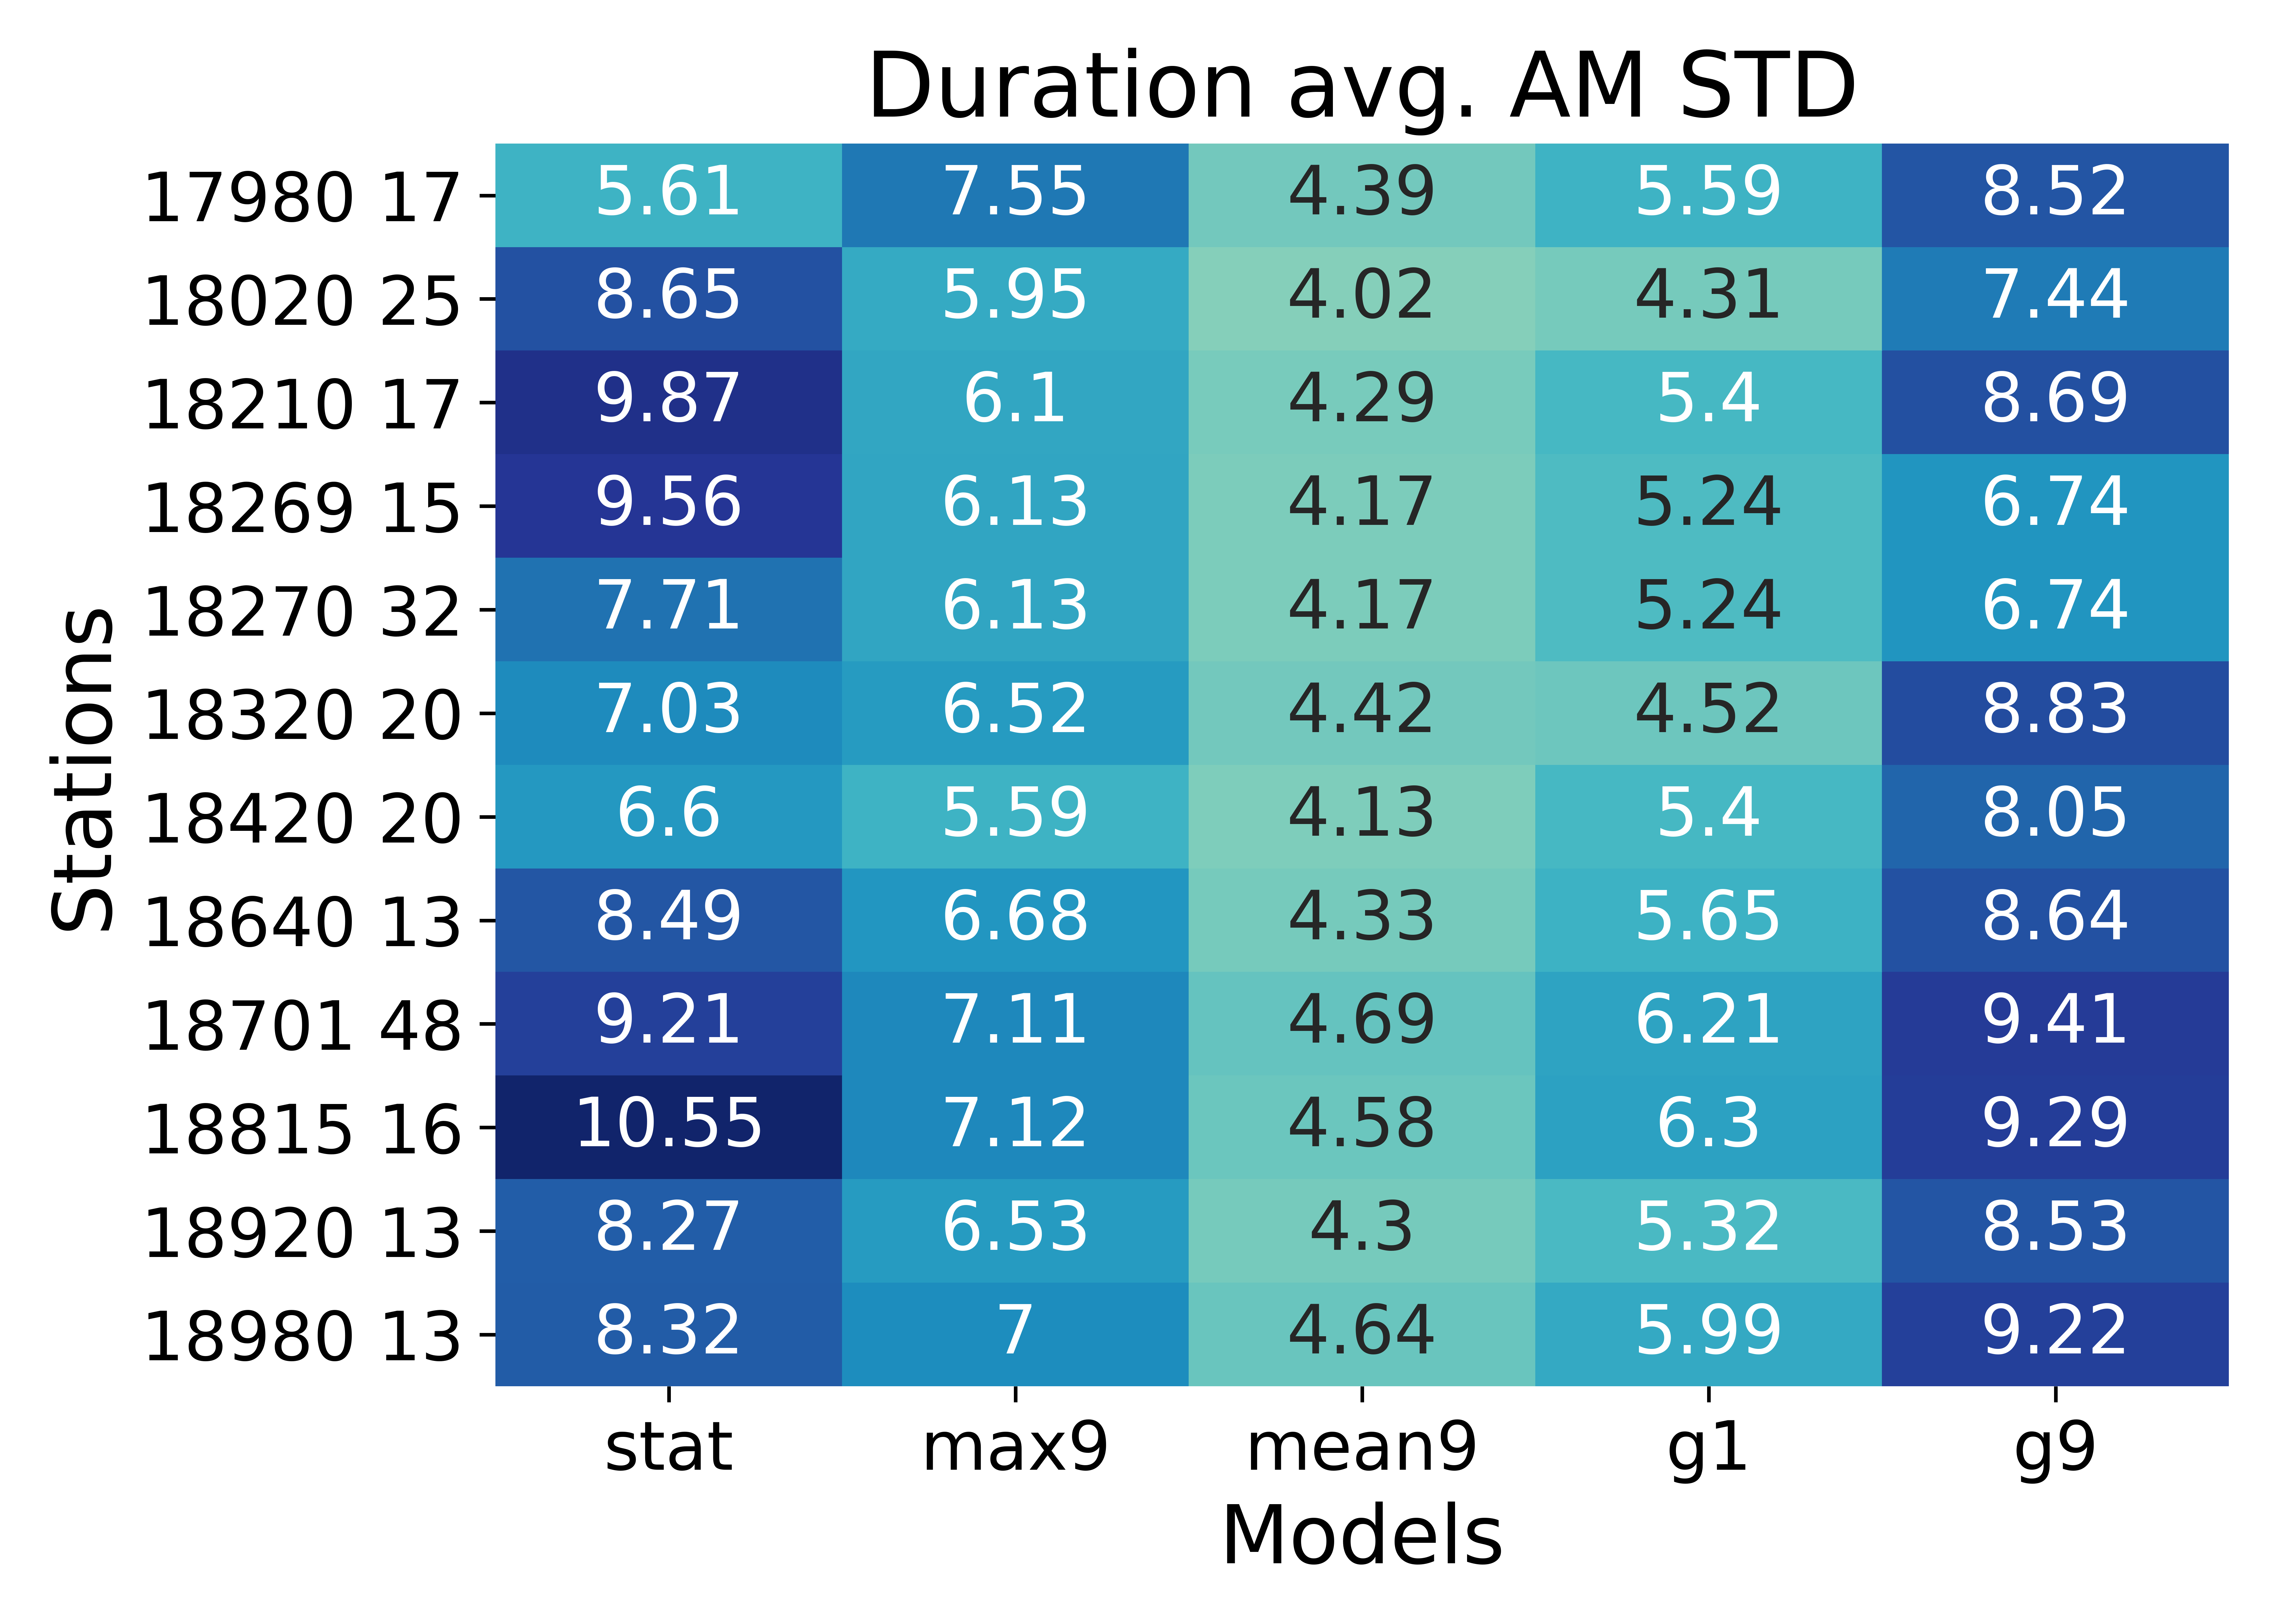
\includegraphics[scale=0.6]{figures/AM_dur_avg_std.png}
    \caption{Duration average variance of annual maximum precipitation data.}
    \label{fig:AM_dur}
\end{figure}

The MEAN method has a very consistent, low STD at around 4 mm across all stations. Also MAX and G1 has low STDs, but the differences between the stations are greater. The largest STD for the MEAN and G9 method are found at station 18701 and the largest for the G1 and STAT are found at station 18815. \textbf{DISCUSSION: 18701 has a long time series while 18815 has a short. Thus its not obvious that the time series length is closely linked to the STD of the AM.}

Figure \ref{fig:AM_stat} shows a heatmap of station average STD of annual maximum precipitation for the different AM methods. All durations are listed on the y-axis while the methods are listed on the x-axis. The first noticeable feature of the plot is the increasing STD with increasing duration across all methods. Only with exception at duration 180 minutes for the G1 method and at 360 minutes for the MAX method the STD are increasing with increasing duration. MEAN has the overall smallest STD with 7.66 mm as maximum value. MAX and G1 has very similar STD across the duration. G9 is the method with STD most similar to STAT.   

\begin{figure}[hbt!]
    \centering
    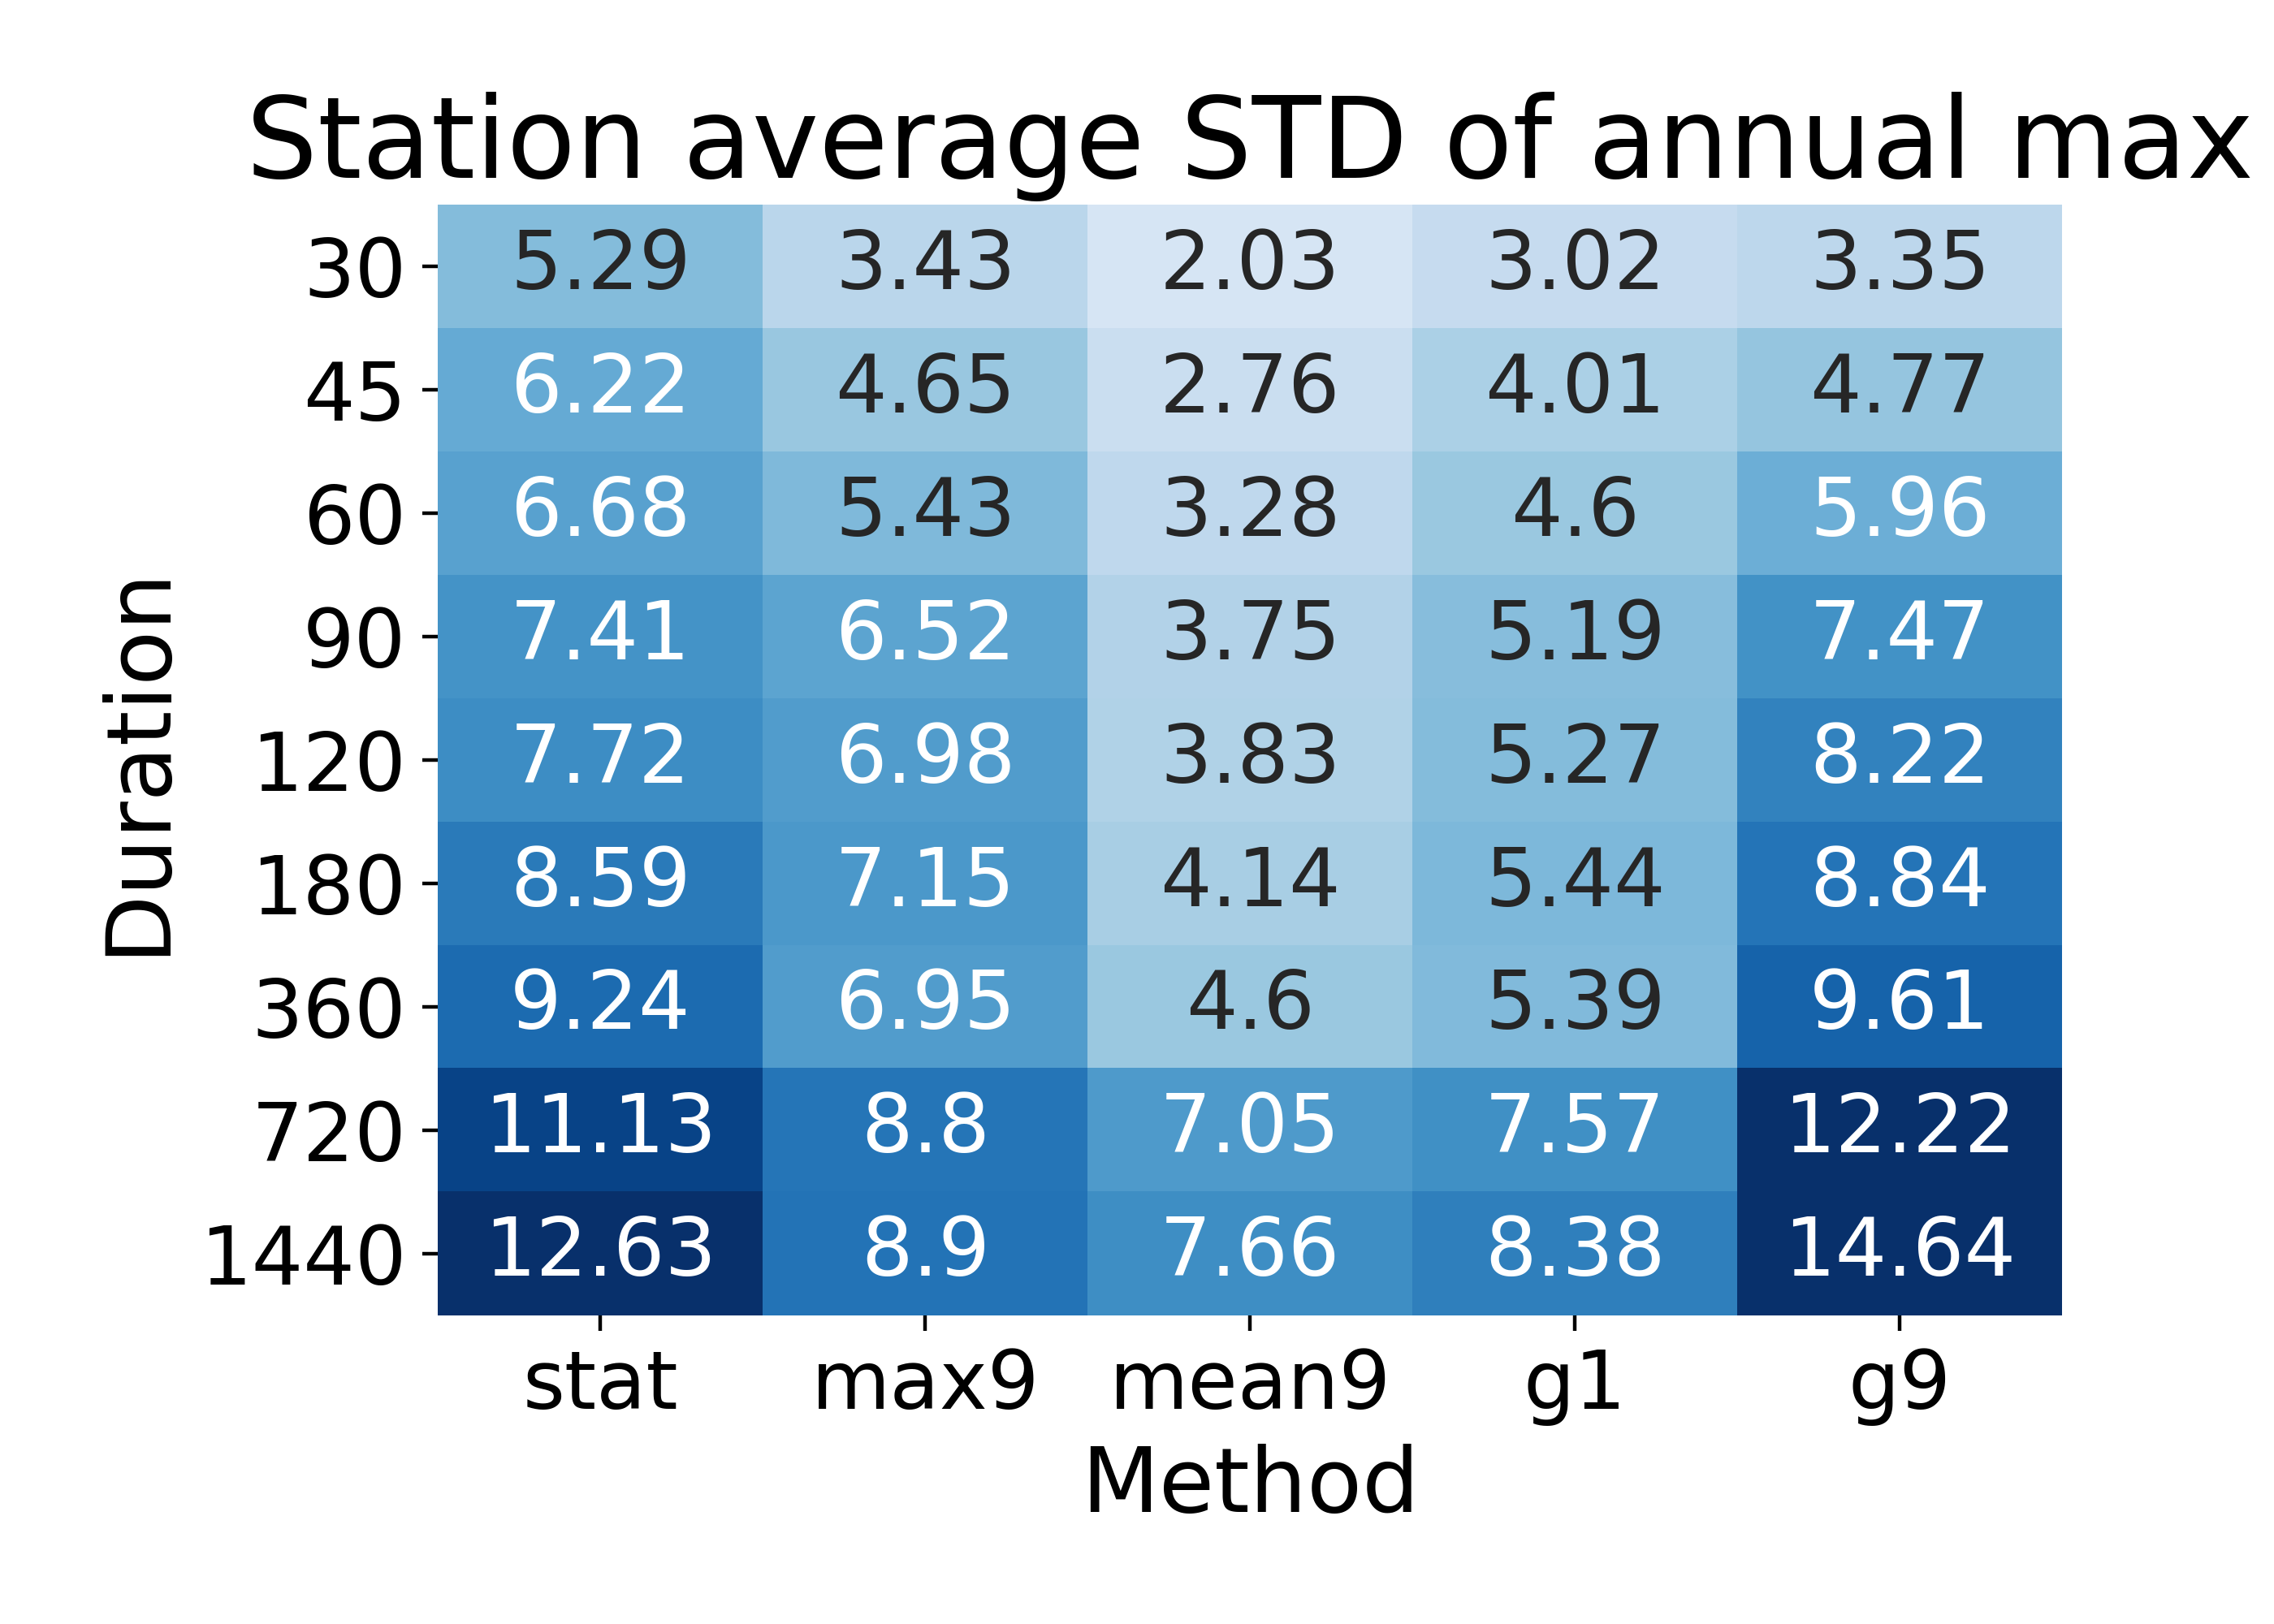
\includegraphics[scale=0.4]{figures/AM_station_avg_std.png}
    \caption{Station average STD of annual maximum precipitation data.}
    \label{fig:AM_stat}
\end{figure}

\subsubsection{Station IDF}

A version of the IDF-curves are presented in Figure \ref{fig:IDF_stat_retper}. Here station-based precipitation magnitude are plotted for all durations at all stations for 2, 20 and 200 year recurrence interval. Despite a relatively short distance between the stations of a few kilometers there are relatively large differences in expected precipitation between them. Station Besserud and station Blindern is only 3km apart, however the 5 year return period return-level at 24h is already more than 10 mm. For the 200 year return period this difference is around 50 mm. In general the difference between high and low return-levels across the stations are larger for larger return periods and smaller for smaller return periods.

\begin{figure}[hbt!]
    \centering
    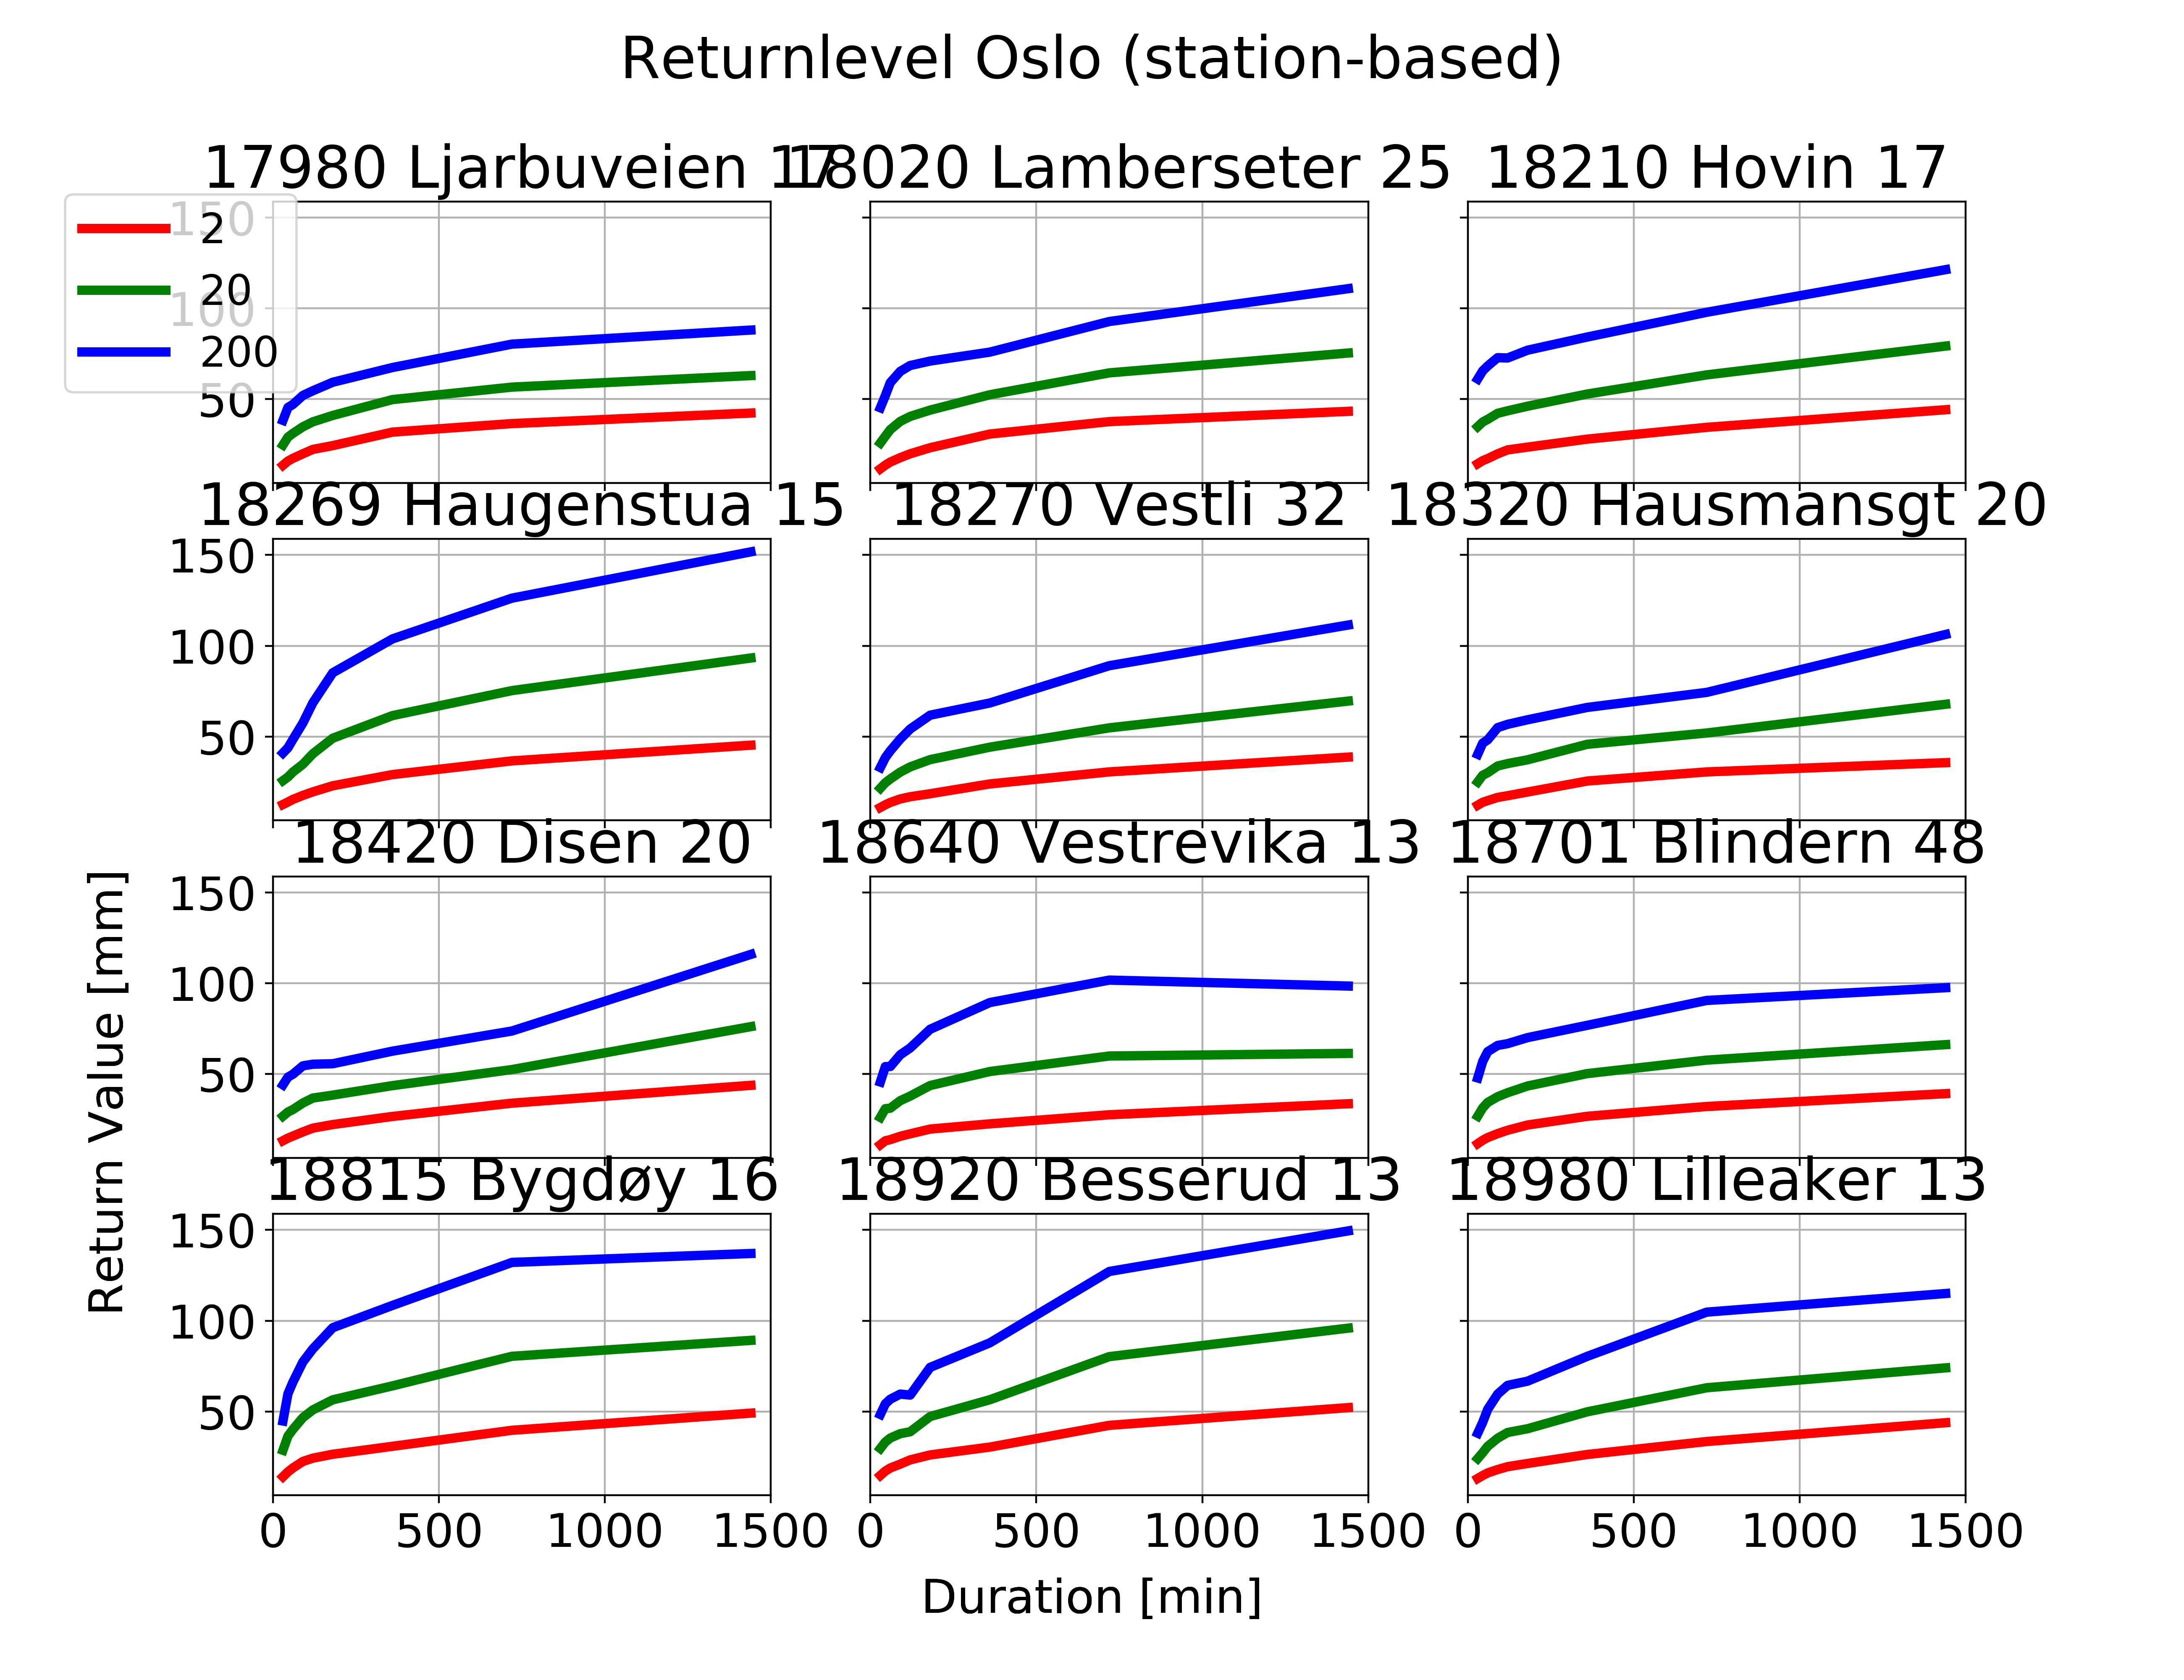
\includegraphics[scale=0.3]{figures/IDF_stat_retper.png}
    \caption{Station average STD of annual maximum precipitation data.}
    \label{fig:IDF_stat_retper}
\end{figure}

Stations like Ljabruvegen and Blindern have a small spread between the 2 year and the 200 year return-level for all durations, while stations like Haugenstua and Besserud has a large spread between the return-levels. The varying station length may contribute to this difference. Blindern has 48 years of data and a small spread compared to Besserud with 13 years of data, thus it appear that the time-series length has a great impact on the spread of the return-levels for each station. On the other hand Ljabruvegen has 17 years of data and a small spread compared to Haugenstua with 15 years of data, so the time-series length is not the only thing affecting the return-levels.   

\textbf{Include figure with real IDF for stat all stations? Like the one above but with intensity} 



\subsubsection{Introducing modelled precipitation}

\subsection{sub malte}

ECE-ERAI: slopes, regimes: convective or stratiform. Should hypothesise this! -> becomes more differnt -> stratiform precipitation more different between ECE and ERAI. 

What is triggering convective preciptiation at BLindern? Why is this different in ECE/ERAI?

What is important driver for stratiform? How much precip is transported into the area? 

Cant disqualifie method based on True/False (confidence), discuss instead. 

Suggestion: Stick to ECE. Drp ERAI, use ECE future instead. Stick to GCM since AROME is GCM. Do not include reanalysis data, complicated for this cliamte model study.

Can bring ERAI in at the end in "what needs to be done"?

\subsection{2080-2100}
